%%%%%%%%%%%%%%%%%%%%%%%%%%%%%%%%%%%%%%%%%
% Classicthesis Typographic Thesis
% LaTeX Template
% Version 1.4 (1/1/16)
%
% This template has been downloaded from:
% http://www.LaTeXTemplates.com
%
% Original author:
% André Miede (http://www.miede.de) with commenting modifications by:
% Vel (vel@LaTeXTemplates.com)
%
% License:
% GNU General Public License (v2)
%
% General Tips:
% 1) Make sure to edit the classicthesis-config.file
% 2) New enumeration (A., B., C., etc in small caps): \begin{aenumerate} \end{aenumerate}
% 3) For margin notes: \marginpar or \graffito{}
% 4) Do not use bold fonts in this style, it is designed around them
% 5) Use tables as in the examples
% 6) See classicthesis-preamble.sty for useful commands
%
%%%%%%%%%%%%%%%%%%%%%%%%%%%%%%%%%%%%%%%%%

%----------------------------------------------------------------------------------------
%	PACKAGES AND OTHER DOCUMENT CONFIGURATIONS
%----------------------------------------------------------------------------------------

\documentclass[
		twoside,openright,titlepage,numbers=noenddot,headinclude,%1headlines,
	 	footinclude=true,cleardoublepage=empty,
		dottedtoc, % Make page numbers in the table of contents flushed right with dots leading to them
		BCOR=5mm,paper=a4,fontsize=11pt, % Binding correction, paper type and font size
		ngerman,american, % Languages, change this to your language(s)
		]{scrreprt} 
                
% Includes the file which contains all the document configurations and packages - make sure to edit this file
\input{classicthesis-config}

\addbibresource{bib/strong2l_paper.bib}
\addbibresource{atlaslatex/bibtex/bib/ATLAS.bib}
\addbibresource{atlaslatex/bibtex/bib/CMS.bib}
\addbibresource{atlaslatex/bibtex/bib/ConfNotes.bib}
\addbibresource{atlaslatex/bibtex/bib/PubNotes.bib}
\addbibresource{Bibliography.bib} % The file housing your bibliography
%\addbibresource[label=ownpubs]{Self_Publications.bib} % Uncomment for optional self-publications

%\hyphenation{Put special hyphenation here}

\begin{document}

\frenchspacing % Reduces space after periods to make text more compact

\raggedbottom % Makes all pages the height of the text on that page

\selectlanguage{american} % Select your default language - e.g. american or ngerman

%\renewcommand*{\bibname}{new name} % Uncomment to change the name of the bibliography
%\setbibpreamble{} % Uncomment to include a preamble to the bibliography - some text before the reference list starts

\pagenumbering{roman} % Roman page numbering prior to the start of the thesis content (i, ii, iii, etc)

\pagestyle{plain} % Suppress headers for the pre-content pages

%----------------------------------------------------------------------------------------
%	PRE-CONTENT THESIS PAGES
%----------------------------------------------------------------------------------------

% Title Page

\begin{titlepage}

%\begin{addmargin}[-1cm]{-3cm}
\begin{center}
\large

\hfill
\vfill

\begingroup
\color{RoyalBlue}\spacedallcaps{\myTitle} \\ \bigskip % Thesis title
\endgroup

\spacedlowsmallcaps{\myName} % Your name

\vfill

A dissertation submitted in partial satisfaction of the \\
requirements for the degree of \\
Doctor of Philosophy \\
in Physics \\
in the Graduate Division \\
of the University of California, Berkeley \\

\vfill

\includegraphics[width=5cm]{gfx/ucberkeleyseal_line_540.eps} \\ 
\bigskip % Picture

Committee in charge: \\
Professor Beate Heinemann, Chair \\
Professor Robert Jacobsen \\
Professor Karl van Bibber \\ \bigskip

Fall 2016

%\mySubtitle \\ \medskip % Thesis subtitle
%\myDegree \\
%\myDepartment \\
%\myFaculty \\
%\myUni \\ \bigskip

%\myTime\ -- \myVersion % Time and version

\vfill

\end{center}
%\end{addmargin}

\end{titlepage} % Main title page

\include{FrontBackMatter/Titleback} % Back of the title page

\cleardoublepage% Dedication

\thispagestyle{plain}
\refstepcounter{dummy}

\pdfbookmark[1]{Dedication}{Dedication} % Bookmark name visible in a PDF viewer

\vspace*{6cm}

\begin{center}
\textit{To my brother for at least starting to lead the way.}
\end{center}

%\medskip

%\begin{center}
%Dedicated to the loving memory of Rudolf Miede. \\ \smallskip
%1939\,--\,2005
%\end{center} % Dedication page

%\cleardoublepage\include{FrontBackMatter/Foreword} % Uncomment and create a Foreword.tex to include a foreword

\cleardoublepage% Abstract

%\renewcommand{\abstractname}{Abstract} % Uncomment to change the name of the abstract

\pdfbookmark[1]{Abstract}{Abstract} % Bookmark name visible in a PDF viewer

\begingroup
\let\clearpage\relax
\let\cleardoublepage\relax
\let\cleardoublepage\relax

\chapter*{Abstract}
A search for new phenomena in final states containing a $Z$ boson decaying to electrons or muons, jets, and large missing transverse momentum is presented. This search uses proton--proton collision data collected during 2015 and 2016 at a center of mass energy $\sqrt{s}=13$~\TeV\ by the ATLAS detector at the Large Hadron Collider, which correspond to an integrated luminosity of \lumi. The search targets the pair production of supersymmetric particles, squarks or gluinos, which decay via jets and a $Z$ boson to the lightest Supersymmetric particle, which does not interact with the ATLAS detector. Results are interpreted in simplified models of gluino-pair (squark-pair) production, and provide sensitivity to gluinos (squarks) with masses as large as~1.3~(1.0)~\TeV.

\endgroup			

\vfill % Abstract page

\cleardoublepage\include{FrontBackMatter/Publications} % Publications from the thesis page

\cleardoublepage% Acknowledgements

\pdfbookmark[1]{Acknowledgements}{Acknowledgements} % Bookmark name visible in a PDF viewer



\bigskip

%----------------------------------------------------------------------------------------

\begingroup

\let\clearpage\relax
\let\cleardoublepage\relax
\let\cleardoublepage\relax

\chapter*{Acknowledgements}

\noindent 

It's difficult to express how important support from my friends has been for me throughout graduate school. Traveling often between Berkeley and Geneva, it would have been easy to never fully feel fully settled in either place. Instead, each time I traveled to CERN, I had an R1 table full of friends waiting for me. Thanks especially to Kate and Max for being truly incredible. And when I returned to Berkeley, Carolyn, Michael, Brad, and Jackie were all there to welcome me back and make me feel at home. And of course, Katayun, I feel like you've been with me through all of it, and I couldn't have made it this far without you.

I've had the privilege of working with incredible people both at Berkeley and at CERN. Thank you to Beate, for always having a birds eye view and keeping me going in the right direction. Thank you to Emma, Jon, and Christian for being delightful to work with. And most of all, thank you to Zach, for everything.

Thank you to my family for being almost absurdly enthusiastic about me still being a student at 27. Mom, I love your curiosity about everything I do. Ben, thank you for always supporting me, and for giving me my first taste of physics. Your collective assuredness that I am on the right track has kept me going, even when I'm far less certain than you are. 

And to Larry, for gracefully filling the roles of supportive boyfriend and nearest postdoc simultaneously. You're the best one.


\endgroup % Acknowledgements page

\pagestyle{scrheadings} % Show chapter titles as headings

\cleardoublepage\include{FrontBackMatter/Contents} % Contents, list of figures/tables/listings and acronyms

\cleardoublepage

\pagenumbering{arabic} % Arabic page numbering for thesis content (1, 2, 3, etc)
%\setcounter{page}{90} % Uncomment to manually start the page counter at an arbitrary value (for example if you wish to count the pre-content pages in the page count)

\cleardoublepage % Avoids problems with pdfbookmark

%----------------------------------------------------------------------------------------
%	THESIS CONTENT - CHAPTERS
%----------------------------------------------------------------------------------------

\ctparttext{The centerpiece of this thesis is a search for Supersymmetry, but it also includes all the scaffolding and background necessary to understand the search. An overview of the \ac{LHC} and the ATLAS Detector are presented along with the theory that motivates the search.} % Text on the Part 1 page describing  the content in Part 1

\part{Introduction} % First part of the thesis

% Chapter 1

\chapter{Introduction} % Chapter title

\label{ch:introduction} % For referencing the chapter elsewhere, use \autoref{ch:introduction} 

%----------------------------------------------------------------------------------------
The pages that follow detail the author's work on the ATLAS experiment from 2011 through 2016, focusing on an analysis of $13 TeV$ proton-proton collisions at the \ac{LHC} looking for Supersymmetry with the ATLAS Detector. 

\paragraph{Chapter 2} outlines the Standard Model of Particle Physics and the benefits of extending it to include Supersymmetry, then continues on to introduce the specific models used in the search presented in later chapters. It also provides an overview of the process of generating \ac{MC} for use in the ATLAS experiment.

\paragraph{Chapter 3} describes the \ac{LHC} and its operation, including the magnet system, the preaccelerator complex, and some of the phenomenology of collisions at 13 \tev.

\paragraph{Chapter 4} contains descriptions of the many pieces of the ATLAS detector, and how they serve to detect particles coming from \ac{LHC} collisions. ATLAS's magnet and trigger systems are also discussed.

\paragraph{Chapter 5} details the process of reconstruction, the procedue by which the electric signals in the ATLAS detector are interpreted as particles to be used for analysis. 

\paragraph{Chapter 6} presents a neural network designed to improve tracking in the ATLAS Pixel Detector, and describes the benefits of its implementation. 

\paragraph{Chapter 7} lists the main backgrounds for the Supersymmetry search described in this thesis, and provides general ideas of how they can be reduced. 

\paragraph{Chapter 8} outlines how objects are identified and selected for this analysis, referencing many of the working points defined in Chapter 5.  

\paragraph{Chapter 9} explains the analysis's search strategy, defining signal, control, and validation regions, and briefly describing how each contributes to the search.

\paragraph{Chapter 10} describes, for each of the backgrounds described in Chapter 7, how estimates of the Standard Model contributions to the signal region are performed. 

\paragraph{Chapter 11} builds off of Chapter 11, and continues to detail how the uncertainties on each estimate are assessed. 

\paragraph{Chapter 12} shows the results of the analysis, comparing expectations based on background estimates to the observed data. 

\paragraph{Chapter 13} provides interpretations of the results, and explains the statistical procedure used to define exclusions on Supersymmetric models. 

\paragraph{Chapter 14} concludes with a summary of the results, and an outlook for future searches. 
 % Chapter 1

\cleardoublepage % Empty page before the start of the next part

%------------------------------------------------

\ctparttext{This section describes the theoretical foundation for the analysis presented in \autoref{part:search}. It includes an overview of the Standard Model, including its phenomenology in a $p-p$ collider. The theory of Supersymmetry is explained, and the motivation for extending the Standard Model to include it is presented. In addition, this section includes an explanation of Monte Carlo generators and details about the specific form of Supersymmetry searched for in this analysis.} % Text on the Part 2 page describing the content in Part 2

\part{Theory and Motivation} % Second part of the thesis

% Chapter 2

\chapter{Theory and Motivation} % Chapter title

\label{ch:theory} % For referencing the chapter elsewhere, use \autoref{ch:examples} 

%----------------------------------------------------------------------------------------

Some kind of preamble here I guess.

%----------------------------------------------------------------------------------------

\section{The Standard Model}

%------------------------------------------------

\subsection{Standard Model Phenomenology}

I will put this off for now.

\subsection{Problems in the Standard Model}

\subsection{Phenomenology of Proton-Proton Collisions}
\subsubsection{Parton Distribution Functions}

%------------------------------------------------

\section{Supersymmetry}

\subsection{Supersymmetry Phenomenology}
\subsection{Solutions to Standard Model Problems}
\subsection{Supersymmetry Signatures in $p-p$ Collisions}
\subsubsection{Simplified Models Used in This Analysis}
\label{sec:simplified_models}

\section{Monte Carlo Generators}
 % Chapter 2

\cleardoublepage % Empty page before the start of the next part

%------------------------------------------------

\ctparttext{This section describes the \ac{LHC} and the ATLAS detector, which collectively provide the physical environment and the data collection for the analysis discussed in \autoref{part:search}.} % Text on the Part 2 page describing the content in Part 2

\part{The Experiment} % Second part of the thesis

% Chapter 3

\chapter{The Large Hadron Collider} % Chapter title

\label{ch:lhc} % For referencing the chapter elsewhere, use \autoref{ch:mathtest}

%----------------------------------------------------------------------------------------

The \ac{LHC} is unique in the world, producing particle collisions at energies an order of magnitude higher than any accelerator before. It provides unique environments in its proton-proton collisions where massive, unstable particles can exist for an instant, then decay to the ordinary material of the universe.

%----------------------------------------------------------------------------------------

\section{Operation of the Large Hadron Collider}

 % LHC
% Chapter X

\chapter{The ATLAS Detector} % Chapter title

\label{ch:atlas} % For referencing the chapter elsewhere, use \autoref{ch:name} 

The \acf{ATLAS} detector circumscribes the \ac{LHC}'s beam pipe, enclosing the collision point with a series of particle detecting layers, aimed at making as many measurements of the particles leaving the collision point as possible. Its goal is to get a precise measurement of all the stable or semi-stable particles flying from proton-proton collisions at its center, allowing analyzers to fully reconstruct the kinematics of the underlying processes.

The \ac{ATLAS} detector is the largest detector of its kind, measuring 44 m in length and 25 m in height, as seen in \autoref{fig:detector}. The size is mainly determined by the constraints of the \acf{MS}, discussed in \autoref{sec:MS}, which is the largest and outermost subsystem. The \ac{MS} is submerged in a spatially varying magnetic field provided by three toroidal magnets, while the \acf{ID} (\autoref{sec:ID}) is encased by a superconducting solenoid, which provides a uniform 2 T field throughout its volume \cite{PERF-2007-01}. A calorimeter system is located between the \ac{MS} and \ac{ID}, with components to measure the energy of electromagnetic and hadronic systems. 

\begin{centering}
\begin{figure}[bth]
\myfloatalign
\includegraphics[width=.90\linewidth]{figures/atlas/detector.pdf}
\caption{Diagram of the \ac{ATLAS} detector, with subsystems and magnets identified.}
\label{fig:detector}
\end{figure}
\end{centering}

\section{Coordinate System Used in the \ac{ATLAS} Detector}
\label{sec:coords}

The \ac{ATLAS} detector is centered around the $pp$ collision point, and is built radially out from the beam pipe, maintaining as much rotational symmetry around the beam pipe as possible. It is also symmetric in the forward-backward directions. A coordinate system using the collision point as the origin is used, with the beam line defining the $z$-axis in the counter-clockwise direction. The positive $x$ direction is defined as pointing to the center of the \ac{LHC} ring, while the positive $y$ direction points upwards. For ease of reference, the side of the detector in the positive-$z$ direction is referred to as the A side, and the other side is referred to as the C side. 

Because of the cylindrical design of the detector, angular coordinates are often used. The azimuthal angle $\phi$ defines the angle around the beam pipe and the polar angle $\theta$ defines the angle from the beam axis ($z$). However, a transformation of the polar angle called pseudorapidity ($\eta$) is used more often, and is defined as 

\begin{equation}
\eta = - \mathrm{ln} [ \mathrm{tan} \frac{\theta}{2} ]. 
\end{equation}

$\eta$ is used because the particle distribution from \ac{LHC} collisions is roughly uniform in this variable. Building on this definition, angular distance between objects is typically defined as

\begin{equation}
\Delta R = \sqrt{\Delta\eta^2 + \Delta\phi^2}. 
\end{equation}

Often variables are defined purely in the transverse plane, which is indicated by a subscripted $T$, as in $p_T$, which gives an object's transverse momentum. 

%------------------------------------------------

\section{The Inner Detector}
\label{sec:ID}

The \acf{ID} is used for the measurement of tracks, estimates of the paths charged particles take as they travel through the detector. Collisions in the detector produce about 1000 particles, so identifying and differentiating all the tracks resulting from a collision is challenging. 

The \ac{ID} consists of three separate subdetectors, each of which has multiple layers capable of producing an electrical signal, called a \textit{hit}, when a charged particle travels through its active material. \ac{ATLAS} tracking software considers all these hits and forms tracks, with the goal of minimizing fake tracks due to random noise and maximizing the efficiency of identifying a real particle. Some details of this procedure are discussed in \autoref{sec:NN}. The full \ac{ID} can be seen in \autoref{fig:ID}, while a schematic in \autoref{fig:IDeta} shows more detail on the placement of each layer.

\begin{centering}
\begin{figure}[bth]
\myfloatalign
\includegraphics[width=.90\linewidth]{figures/atlas/innerdetector.pdf}
\caption{Diagram of the \ac{ATLAS} Inner Detector, containing the Pixel, SCT, and TRT subsystems.}
\label{fig:ID}
\end{figure}
\end{centering}

\begin{centering}
\begin{figure}[bth]
\myfloatalign
\includegraphics[width=.90\linewidth]{figures/atlas/ideta.pdf}
\caption{Diagram of one-quarter of the \ac{ATLAS} Inner Detector in the $R-z$ plane, with lines drawn to indicate various $\eta$ locations.}
\label{fig:IDeta}
\end{figure}
\end{centering}

\subsection{The Pixel Detector}

The pixel detector lies closest to the beam pipe of the \ac{LHC}, and has four layers comprising 92 million pixels. There are three standard layers, referred to as Layers 0-2 (L0, L1, L2), and an additional layer added for the 2015 data-taking, called the \ac{IBL}. 

\subsubsection{The Original Pixel Detector}

The Pixel Detector consists of high-precision silicon chip pixel modules, with 1744 in total, and each module is made up of 16 sensors each with its own read-out system. Each sensor is identical, containing 47232 pixels, which are typically each 50$\times$400 $\mu$m$^2$, though pixels at the edges of the sensors are slightly longer, at 50$\times$600 $\mu$m$^2$.  

As shown in \autoref{fig:IDeta}, the central $\eta$ region (barrel) is covered by three concentric cylindrical layers of sensors with radii of 50.5 mm, 88.5 mm, and 122.5 mm. In the higher $\eta$ region (endcap) is covered by a series of three disks positioned in the $x-y$ plane. Together, they give complete coverage out to $|\eta| = 2.5$, and a particle coming from the collision point will typically produce hits in three layers. 

The sensors are n-type silicon wafers with a voltage applied, and a passing charged particle produces thousands of electron-hole pairs inside the material, which drift in the electric field towards the mounted read-out system. A hit occurs when the resulting current becomes large enough to pass a threshold designed to suppress noise. A larger total charge deposit will result in the signal remaining over the threshold for a longer period of time. This \ac{ToT} is recorded along with the initial timing of the hit. This measurement is spatially accurate in the barrel (endcap) to 10 $\mu$m in the $R-\phi$ direction and 115 $\mu$m in the $z$ ($R$) direction.  

\subsubsection{Addition of the IBL}

In 2014, the \ac{IBL} was added to the Pixel Detector. This layer is placed directly on top of the beam pipe, inside barrel L0, providing a measurement of particles only 3.3 cm away from the interaction point. The \ac{IBL} consists of 14 overlapping staves, each containing 16 modules, the geometry of which can be seen in \autoref{fig:ibl_add}. These modules contain pixels measuring 50$\times$250 $\mu$m$^2$, and allow for particle detection in 90\% their area, as compared to the 70\% possible with the original pixel modules.

\begin{centering}
\begin{figure}[bth]
\myfloatalign
\includegraphics[width=.90\linewidth]{figures/atlas/IBL-other.png}
\caption{Diagram in the $x-y$ plane of the \ac{IBL} and the innermost layer of the pixel detector, L0 \cite{1201.5469}.}
\label{fig:ibl_add}
\end{figure}
\end{centering}

The \ac{IBL}'s addition provides greater precision for all track measurements, but it is especially useful for the detection of $B$ mesons, discussed in \autoref{sec:quarks}, whose lifetimes of about 1.5 ps allow them to travel as much as a few mm before decaying. These decays lead to secondary vertices in \ac{ATLAS} events. The location of the \ac{IBL} gives a measurement closer to these secondary vertices, increasing the probability that these vertices can be resolved. 

\subsection{The Silicon Microstrip Tracker}

The \ac{SCT} employs a similar technology to the Pixel Detector, with 15912 sensors and 6.3 million readout channels. Its main difference from the Pixel Detector is in the readout, which is performed by a series of 12 cm long strips with a width of 80 $\mu$m. These layers are paired, placed on top of one another at a small (40 mrad) angle to allow for position determination in the $\phi$ and $z$ directions. Together, these pairs of layers give four spatial measurements for each particle passing through the \ac{SCT}. In the barrel, these strips run parallel to the beam pipe, while in the endcap, they are arranged radially. These strips provide a hit resolution in the barrel (endcap) of 17 $\mu$m in the $R-\phi$ direction and 580 $\mu$m in the $z$ ($R$) direction. 

\subsection{The Transition Radiation Tracker}

The \ac{TRT} uses 4 mm diameter gas-filled tubes, each with a high voltage wire suspended along the center of the tube. The tubes run the length of the barrel, with a separate wire in the positive and negative $z$ direction. In the endcap, the tubes are arranged radially. In total, there are about 351,000 readout channels in the \ac{TRT}. This detector makes measurements only in the $R-\phi$ direction, where the resolution of each measurement is 130 $\mu$m, and coverage extends to $|\eta|=2.0$. Each particle typically creates about 36 hits as it passes through the \ac{TRT} barrel. 

Particles passing through the gas mixture of the \ac{TRT} ionize the gas, producing electrons which drift towards the wire due to a potential difference applied between it and the tube. In addition, particles passing through the \ac{TRT} produce radiation as they transition between materials, with larger amounts of radiation for lighter particles. This radiation produces high-threshold signals in the \ac{TRT} can be used to differentiate electrons from other heavier charged particles, such as pions. 


\section{The Calorimeters}
\label{sec:Calo}

Unlike the tracking detectors, which aim to take measurements of a particle with minimal alterations of its trajectory, the calorimeters measure the energy of objects by stopping them entirely. Calorimeters contain alternating layers of absorber, a material that causes incoming particles to shower into lower-energy decay products, and an active material, which detects passing particles, allowing for the reconstruction of these showers.

The \ac{ATLAS} calorimeters, which can be seen in \autoref{fig:calo}, provide coverage out to $|\eta| < 4.9$. High granularity electromagnetic measurements are made within $|\eta| < 2.5$. In this range, high-\pt electrons have nearly straight tracks, making momentum measurement through track curvature difficult, leaving the calorimeter as the primary energy measurement. The hadronic calorimeters, as well as the higher $|\eta|$ electromagnetic calorimeters, have a coarser granularity. 

\begin{centering}
\begin{figure}[bth]
\myfloatalign
\includegraphics[width=.90\linewidth]{figures/atlas/calorimeters.pdf}
\caption{The calorimeter system of the \ac{ATLAS} detector.}
\label{fig:calo}
\end{figure}
\end{centering}

Besides measuring the energy of passing particles, another task of the calorimeter system is to limit punch-through to the \ac{MS}, described in \autoref{sec:MS}. All other particles must be fully stopped by the calorimeters to allow for clean signals from muons, and to measure the total energy of the particle. This requirement sets a minimum number of interaction lengths for each of the calorimeters. 

\paragraph{The LAr Electromagnetic Calorimeter} uses liquid argon as its active detector medium alternating with layers of lead acting as the absorber. Signals are read out with capacitively coupled copper plates. The layers are shaped like accordions, which allows for complete coverage with multiple layers of active material, three in central $\eta$ ($0<|\eta|<2.5$) and two at higher $\eta$ ($2.5 < |\eta| < 3.2$). \autoref{fig:calo_mod} shows the layout of a central $\eta$ module, including this accordion-like layering. At $|\eta| < 1.8$, an instrumented liquid argon presampler provides a measurement of energy lost prior to reaching the calorimeters. The total energy resolution for this detector is about 10\%/$sqrt{E}$, with an additional constant term of 0.2\%. 

\begin{centering}
\begin{figure}[!htb]
\myfloatalign
\includegraphics[width=.90\linewidth]{figures/atlas/LARG3-TDR-barrelM_samplings_presamp_new.png}
\caption{Layout of the LAr calorimeter module at central $\eta$ \cite{PERF-2007-01}.}
\label{fig:calo_mod}
\end{figure}
\end{centering}

\paragraph{The Tile Calorimeter} is a hadronic calorimeter which surrounds the LAr Calorimeter. It uses layers of steel as its absorber with scintillating tiles as the active material between them, which are read out by photomultiplier tubes. The Tile Calorimeter covers $|\eta| < 1.7$ with a typical energy resolution of about 50\%/$sqrt{E}$ with a constant term of 5\%. 

\paragraph{The LAr Hadronic Endcap Calorimeter} covers the hadronic calorimetery for higher $\eta$. It uses liquid argon active material and copper plate absorbers, resulting in an energy resolution of approximately 70\%/$sqrt{E}$ with a constant term of 5\%. This calorimeter covers $1.5 < |\eta| < 3.2$, overlapping with the hadronic calorimeters in either direction of its $\eta$ range. 

\paragraph{The FCal} or forward calorimeter provides electromagnetic and hadronic coverage at very high $\eta$ ($3.1 < |\eta| < 4.9$). This calorimeter also uses liquid argon as its active material, and uses copper-tungsten as the absorber. Its energy resolution is about 70\%/$sqrt{E}$ with a constant term of 3\%.

\section{The Muon Spectrometer}
\label{sec:MS}

The \acf{MS} measures charged particles that penetrate the calorimeter system. Because the calorimeters are designed to completely absorb electrons, photons, and hadrons, the \ac{MS} mainly detects muons, which pass through the calorimeter with very little loss of energy. The goal of the \ac{MS} is to give a high-precision measurement of these muons, and also to be able to quickly identify events with muons for the sake of triggering, discussed in \autoref{sec:Trigger}. The layout of the \ac{MS} can be seen in Figures~\ref{fig:muon_xy} and~\ref{fig:muon_rz}. Muons can be measured for all $|\eta|$<2.7, and they can be triggered on for $|\eta|$<2.4. The entire system is about 24 m tall and 40 m long. 

\begin{centering}
\begin{figure}[bth]
\myfloatalign
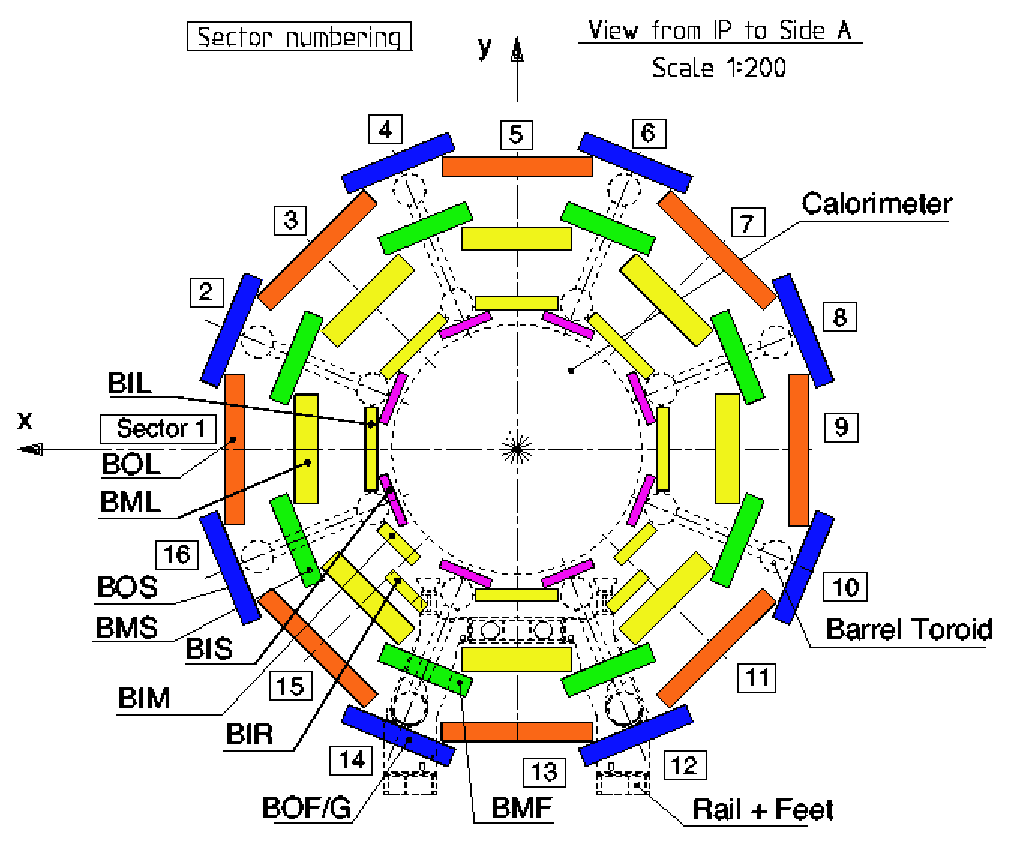
\includegraphics[width=.90\linewidth]{figures/atlas/Muon_sector_numbering.eps}
\caption{An $x$-$y$ view of the \ac{MS}. The three barrel layers are visible, as well as the overlapping, differently sized chambers. The outer layer of the \ac{MS} is about 20m in diameter.}
\label{fig:muon_xy}
\end{figure}
\end{centering}

\begin{centering}
\begin{figure}[bth]
\myfloatalign
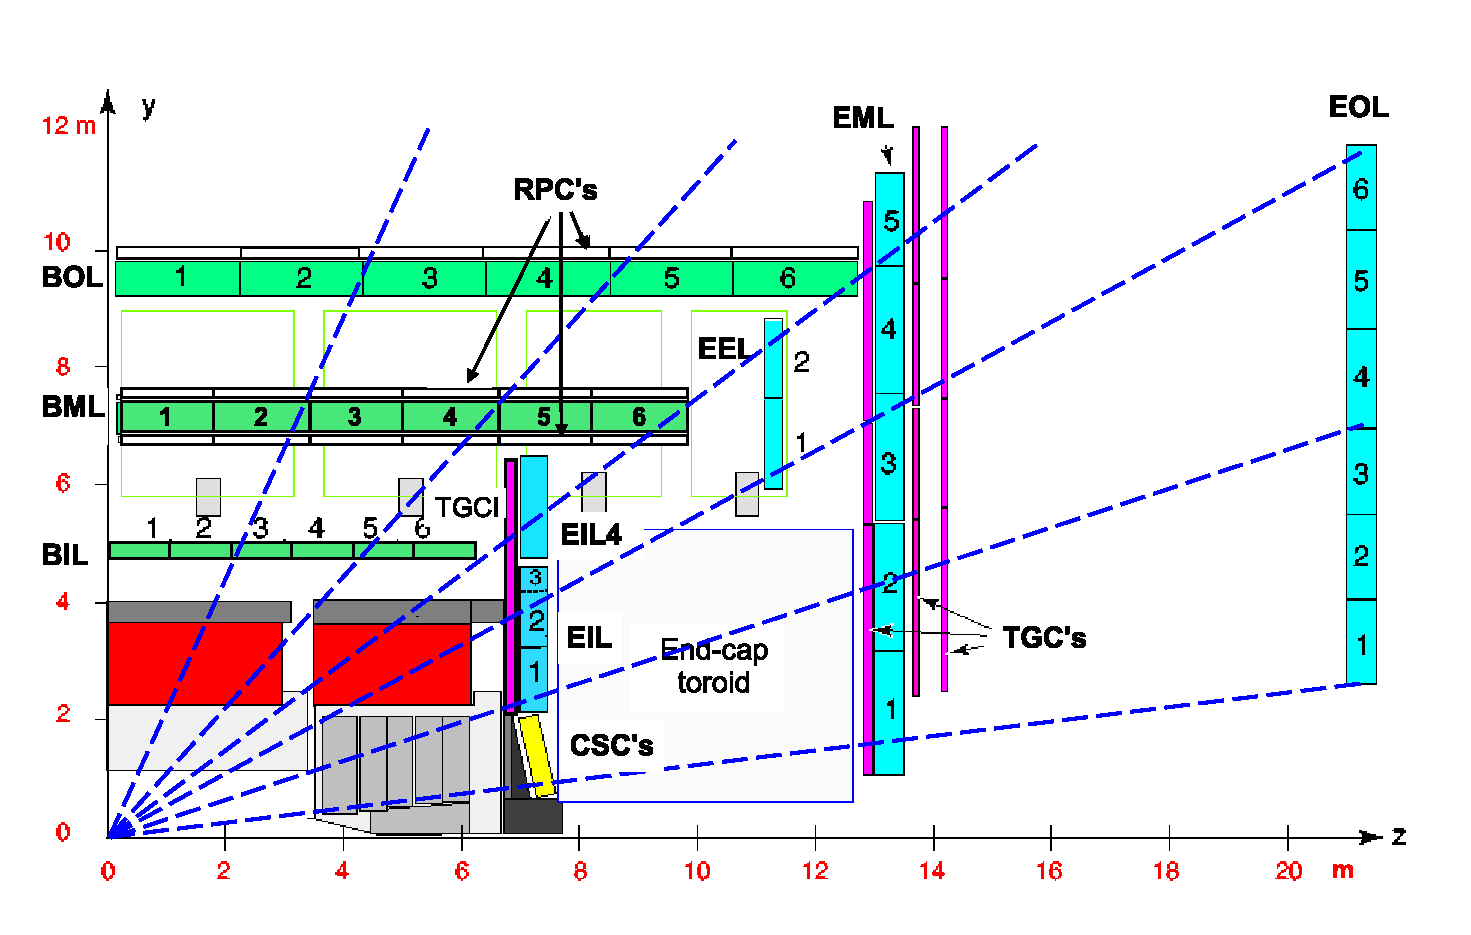
\includegraphics[width=.90\linewidth]{figures/atlas/Muon_rz_large_sect_6.eps}
\caption{An $r$-$z$ view of the \ac{MS}. The three layers of the barrel and endcap \ac{MS} are visible.}
\label{fig:muon_rz}
\end{figure}
\end{centering}

To achieve these goals, the \ac{MS} has several subsystems. The system responsible for precision measurement is called the \acfp{MDT}. This subdetector consists of chambers of three to eight layers of tubes, with three layers of chambers covering both the barrel and endcap regions. In the barrel, these chambers are arranged in layers concentric cylinders with small overlaps between adjacent chambers. The chambers are oriented such that the drift tubes are parallel to the beam line. In the endcap, the chambers form disks with drift tubes approximately aligned in the $R$ direction. 

The tubes each contain an Ar/CO$_2$ gas mixture and a single high voltage wire which runs at its center along its length. Charged particles excite the gas as they pass through it, producing electrons which drift towards the high voltage wire. The resulting electric signal is read out, and the magnitude and timing of the signals are both used to differentiate particle traces from noise. 

Though very effective at giving a precise measurement, the \acp{MDT} have two shortcomings. The first is that the measurement is only precise in the direction perpendicular to the tubes; in the direction parallel to them, the resolution is not much better than the length of the drift tube, which are typically several meters long. The resolution in the perpendicular direction is about 35 $\mu$m with the combined measurement of all the tubes in a chamber. The second major shortcoming is that the \acp{MDT} are slow, with a maximum drift time of about 700 ns. 

The slow drift time means that muons from sequential collisions can appear in the same event, and that the signals from the \acp{MDT} are received too late to be used for triggering. To solve the former problem, another detector called the \acp{CSC} is used in high-rate regions of the \ac{MS}. This detector consists of multi-wire proportional chambers which have cathode strips on either side of the anode in orthogonal directions, providing a 40 $\mu$m resolution in one direction and 5mm resolution in the other. Their drift times are much shorter than those of the \acp{MDT}, at about 40 ns. They are placed in the forward region of the detector (2<$|\eta|$<2.7) where the incident particle rates are highest. 

To achieve responses fast enough to be used for triggering, \acp{RPC} and \acp{TGC} are used. These chambers both take less than 25 ns to produce a signal. The \acp{RPC} are used in the barrel and are made up of two high-resistance plastic plates with a gas mixture under an electric field between them. Passing particles ionize this gas, and the resulting signal is read out via metallic strips mounted to the plastic plates. The \acp{TGC} used in the endcap are a form of multi-wire proportional chambers, like the \acp{CSC}. Unlike the \acp{CSC}, the cathode is placed extremely close to the wires, speeding up its operation. 

The massive \ac{MS} is subject to deformations due to gravity and the magnetic field. To achieve a high precision alignment, these deformations are constantly monitored in each \ac{MDT} chamber with a set of four optical alignment rays, which give alignment information at the precision of <30 $\mu$m. In addition, a sag-adjustment system can use this information to re-align any wires that droop under gravity's pull. Lastly, the \ac{MS} can be aligned using the tracks made from hits it measures, discussed more in \autoref{sec:reco_muons}.

\section{The Magnet System}
\label{sec:magnets}

The \ac{ATLAS} magnet system consists of four superconducting magnets: an inner solenoid, a barrel toroid, and two endcap toroids. Collectively, they are 22m in diameter and 26m long, and their basic layout can be seen in \autoref{fig:magnets}.

\begin{centering}
\begin{figure}[bth]
\myfloatalign
\includegraphics[width=.90\linewidth]{figures/atlas/ATLcoilGeom.eps}
\caption{The magnet system of the \ac{ATLAS} detector. The inner cylinder shows the solenoid which gives a uniform magnetic field in the \ac{ID}. Outside of that are the barrel and endcap toroids, which provide a non-uniform magnetic field for the \ac{MS}.}
\label{fig:magnets}
\end{figure}
\end{centering}

The solenoid is inside the calorimeter volume and provides a uniform 2T magnetic field for particles traveling through the \ac{ID}. This axial field causes the trajectories of charged particles to bend in the $x-y$ plane, and measurements of the curvature of these trajectories give the most accurate \pt measurement for many particles according to the equation

\begin{equation}
\pt = qB\rho 
\end{equation}

where $q$ is the charge of the particle, $B$ is the magnetic field in the $z$ direction, and $\rho$ is the radius of curvature. 

Because the solenoid is placed between the tracking system and the calorimeter, it is important that it interfere minimally with particles in order to allow the calorimeter to measure their full energies. The solenoid is placed inside the same vacuum chamber as the LAr calorimeter and is made of Al-stabilized NbTi superconductor with aluminum casing, giving it a total thickness of about 0.66 radiation lengths. 

The barrel toroid is outside the calorimeters and provides the magnetic field for the barrel \ac{MS}, which varies from 0.2–2.5T. The endcap toroids have a magnetic field range of 0.2-3.5T. All three toroid magnets are made with Al-stabilized Nb/Ti/Cu superconducting coils supported by Al-alloy struts. 

The magnets are cooled with liquid helium, and take up to a month to be brought down to operating temperatures, about 4.5 K. All magnets have cold masses surrounding them to absorb heat in the event of a quench. 

The $B$-field resulting from this magnet system can be seen in \autoref{fig:bfield}. The plot on top demonstrates the relatively constant field rate within the barrel which drops steeply at $|z|$=2. The bottom plot shows the field integral in the \acp{MDT} as a function of $|\eta|$, demonstrating the good coverage out to $|\eta|$<2.6 excluding a transition region between the barrel and endcap, where the field changes rapidly, making precise \pt construction difficult. 

\begin{centering}
\begin{figure}[!htb]
\myfloatalign
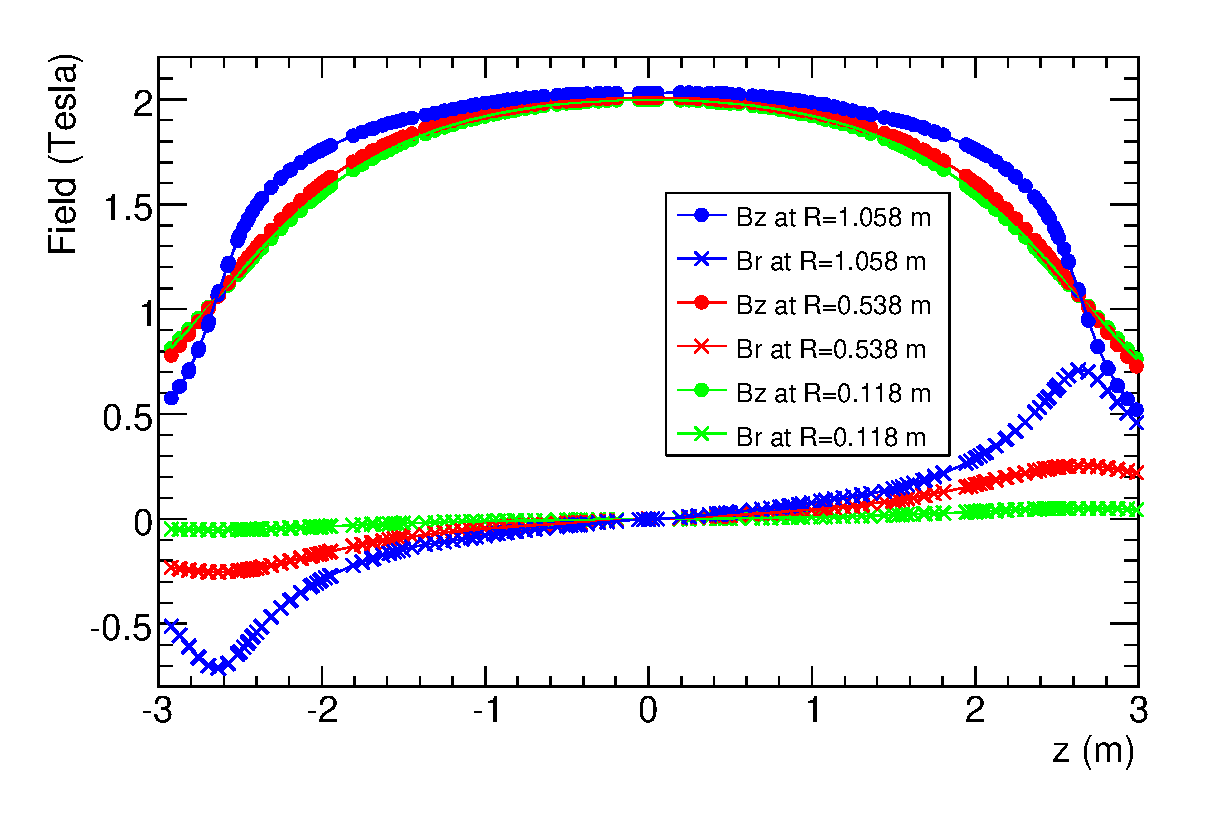
\includegraphics[width=.90\linewidth]{figures/atlas/solMeasB.eps}
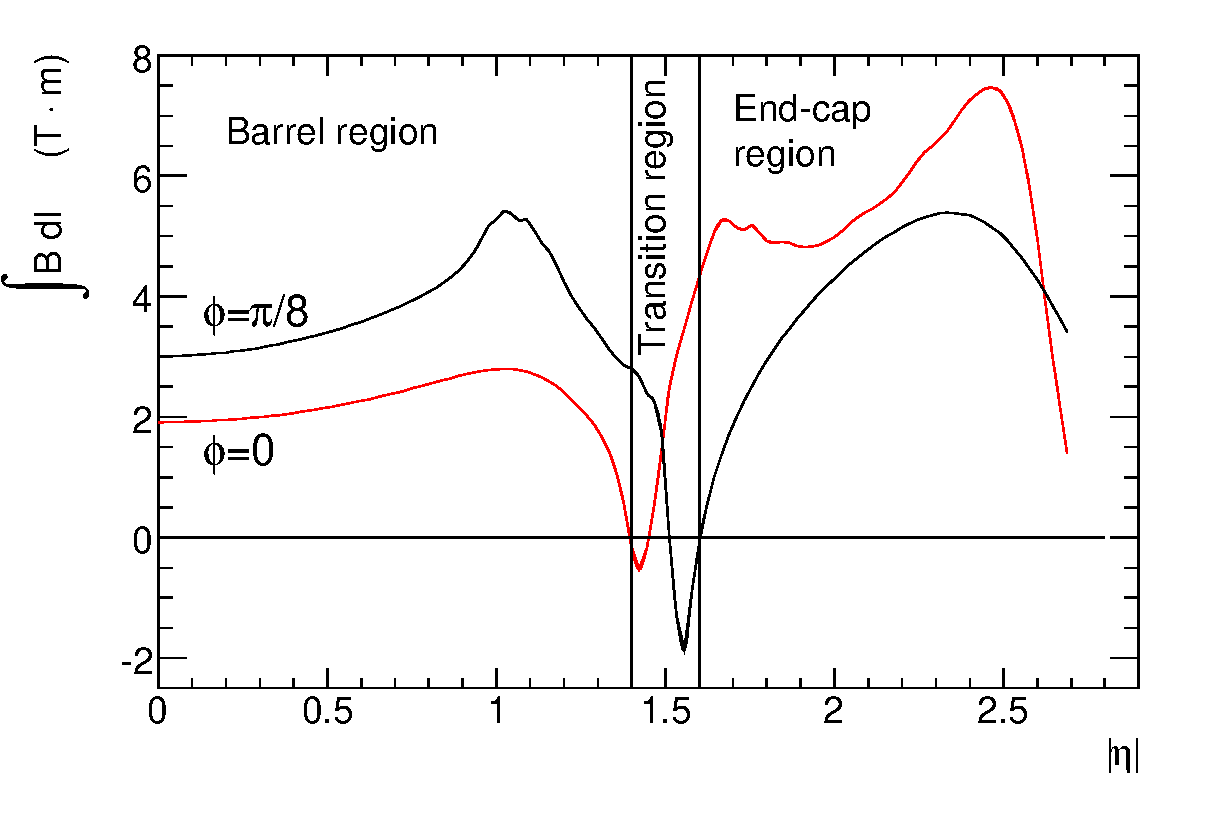
\includegraphics[width=.90\linewidth]{figures/atlas/IBdl.eps}
\caption{Plots of the magnetic field within the \ac{ATLAS} detector. Top is the field (broken into its $R$ and $z$ components) as a function of $z$ for several different values of $R$. Bottom is the field integral through the \acp{MDT} as a function of $|\eta|$ for two different $\phi$ values. }
\label{fig:bfield}
\end{figure}
\end{centering}

\section{The Trigger System and Data Acquisition}
\label{sec:Trigger}

The \ac{LHC} provides proton bunch crossings every 25 ns, and each of these events contains about one MB of data, corresponding to 40 TB/s\footnote{ This number is actually an overestimate, as not all bunches are filled due to the gaps produced by the \ac{LHC}'s injector complex, discussed in \autoref{sec:lhc_inj}.}, a completely unmanageable amount of data. In addition to this concern, many of \ac{ATLAS}'s subdetectors like the Pixel Detector, the LAr Calorimeter, and \acp{MDT} take much longer than 25 ns to read out, making keeping up with the bunch crossing rate impossible. To reduce the total data read out and allow for selective reading out of the slower detectors' buffers, a triggering system is used. 

The trigger system uses fast detectors to get a coarse picture of an event's topology, which is then compared to a trigger menu, which lists the types of events that are interesting enough to keep. Overall, the trigger system reduces the 40 million events a second to about 1000 to be fully read out from the \ac{ATLAS} detector. 

This filtering of events is done in two steps: the \ac{L1} trigger is implemented in hardware and reduces the initial 40MHz to 100kHz, while the \ac{HLT} is implemented in software, further reducing the rate to 1kHz \cite{ATL-DAQ-PUB-2016-001}. The \ac{L1} trigger uses coarse granularity information from the fast read-out subdetectors: the calorimeters, the \acp{RPC} and \acp{TGC}. 

The coarse grained calorimeter information used for the \ac{L1} trigger decision is referred to as \ac{L1Calo} and uses information from all calorimeter systems. \ac{L1Calo} is responsible for all triggers excluding muons, meaning it must be capable of identifying a large number of different objects and event topologies, including high-\pt objects, \met, and large amounts of hadronic energy. The trigger can also identify isolated objects, objects with very few calorimeter deposits from other objects near them.

For muon triggers, the trigger algorithm looks for patterns of hits from the \ac{RPC} and \ac{TGC} that are consistent with high-\pt muons with origins at the interaction point. 

An example of the \ac{L1} trigger rates for different types of events can be seen in \autoref{fig:l1_rates} for one run in July 2016. The common features to all rates are due to \ac{LHC} luminosity changes, deadtimes due to detector inefficiency, and adjustment of trigger rates to optimize bandwidth.

\begin{centering}
\begin{figure}[!hbt]
\myfloatalign
\includegraphics[width=.90\linewidth]{figures/atlas/Time_L1GroupRate_Stack_2016_07.png}
\caption{\ac{L1} trigger rates for for a run in July 2016 as a function of luminosity block, an approximately 60-second long period of data-taking. The total rate is lower than the combined stack because of overlapping triggers.}
\label{fig:l1_rates}
\end{figure}
\end{centering}

%The outputs from the different calorimeters and the \ac{MS} can also be combined with a system called \ac{L1Topo}. Using this, triggers can require more complex topologies, and can suppress backgrounds by as much as a factor of two. 

All of this information is analyzed by the \ac{CTP}, which uses a trigger menu identifying all types of events to be kept to return a trigger decision. Due to the limited size of detector buffers, the event must be processed in about 2.5 $\mu$s. This ensures that the information to be read out has not yet been overwritten when the trigger decision is made. This decision is passed to the \ac{TTC}, which communicates with all subdetectors. Upon receiving a \ac{L1} trigger, the subdetectors read out all the information they've stored about the event and place it on their \acp{ROB}.

The \ac{HLT} takes the data from particular \acp{RoI}, areas containing interesting objects that caused the \ac{L1} trigger. With a more complete picture of the hits observed by the detector, tracks are formed, and the \ac{HLT} can use all of this information to determine whether or not the event is still interesting enough to keep. This process has its own trigger menu with dedicated \ac{L1} seeds for each item. \ac{HLT} triggers typically have slightly higher thresholds than their corresponding \ac{L1} triggers to ensure that events that would pass the \ac{HLT} requirements are very likely to have passed the \ac{L1} requirements. \autoref{fig:hlt_rates} shows the \ac{HLT} rates for the same run in July. In addition to the event types seen in \autoref{fig:l1_rates}, the \ac{HLT} can also identify events with $b$-jets, differentiate between electrons and photons, and identify events interesting for B-physics. 

\begin{centering}
\begin{figure}[!hbt]
\myfloatalign
\includegraphics[width=.90\linewidth]{figures/atlas/Time_HLTGroupRate_Stack_2016_07.png}
\caption{\ac{HLT} trigger rates for for a run in July 2016 as a function of luminosity block, an approximately 60-second long period of data-taking. The total rate is lower than the combined stack because of overlapping triggers.}
\label{fig:hlt_rates}
\end{figure}
\end{centering}


Events passing the \ac{HLT} trigger are written to disk to be analyzed. An example of the total trigger efficiency for single electron triggers is shown in \autoref{fig:trig_el_eff}. %Trigger efficiencies can be taken directly from \ac{MC}, and are measured in data via a method called tag-and-probe, the main principles of which are discussed in \autoref{sec:bg-fake}.

Events types that occur very frequently, such that it would require too much of the total trigger bandwidth to record all events passing a given threshold, are prescaled. Events passing these triggers are only recorded a fraction of the time, and these prescaling rates are used to weight events passing these triggers when they are analyzed. For example, the lowest unprescaled single electron trigger in 2016 data-taking required an electron with \pt of 60 \gev. A trigger requiring electrons with \pt of only 10 \gev~also exists, but only one in ten events passing this trigger is recorded. 

\begin{centering}
\begin{figure}[!hbt]
\myfloatalign
\includegraphics[width=.90\linewidth]{figures/atlas/plot_Combined_Pt_LOGaxis_Et_log_25l_35l_120l_140l.pdf}
\caption{Photon trigger efficiency as a function of \et for four different \ac{HLT} triggers with photon \pt requirements of 25, 35, 120, and 140 \gev~\cite{egamma_trig}.}
\label{fig:trig_el_eff}
\end{figure}
\end{centering}


\section{Monte Carlo Event Generation}
\label{sec:MC_gen}

The complex events of the \ac{LHC} are difficult to model, but modeling them is crucial to analyzers' understanding of \ac{SM} backgrounds and potential signals. To simplify the modeling process, particle interactions are broken down into very small steps, each with associated probabilities of various outcomes. This modeling method is called \acf{MC}, and, at the \ac{LHC} it is broken into several larger steps which are each handled by different software. 

The first step, discussed in \autoref{sec:pp_collisions}, is to determine the energies of the initial particles in a collision, which are provided by several different \ac{PDF} sets. These distributions come from experimental measurements, though there is some variation between different sets. Three different sets are used in this analysis: NNPDF2.3LO \cite{Ball:2012cx} and NLO CT10 \cite{Lai:2010vv} for background and signal processes, and MSTW 2008 \cite{0901.0002} for pile-up events, discussed more in \autoref{sec:pileup}. 

With the initial states of the constituents of the protons described by these probabilistic models, the next step is to model the hard scattering process resulting from the interaction of two of these particles. This is accomplished by a generator, which calculates the cross-sections of the Feynman diagrams of a given process. In particular, these generators typically produce matrix elements, which describe the probability to go from an initial to final state via a hard scattering, including the kinematic properties of the final state. The generator uses these matrix elements to assign one of these hard scattering final states to each event. These hard scattering outputs are then passed to the next step, where parton showering, hadronization, and final and initial state radiation can occur.

Because these matrix elements must be calculated for each event's specific kinematic properties, it can be very computationally intensive, especially when the calculations are performed at very high order. To save computational time, matrix elements are sometimes calculated at a lower order, and later, the total cross-section for a given process can be calculated at a higher order and used to scale the overall number of events generated for the process. These calculations can also be tuned, varying parameters in the generation to create outputs that most closely match experimental data. 
  
%In some cases, this can mean that a tune might include values for certain physical quantities that are different from their measured values because this configuration ultimately produces a result more similar to data. 

Examples of generators include {\sc MadGraph5\_aMC@NLO} \cite{Alwall:2014hca}, {\sc Powheg Box} \cite{PowhegBOX1,PowhegBOX2,PowhegBOX3}, and \sherpa~\cite{sherpa}. Each has different strengths and is used to describe processes that best match those strengths. {\sc Powheg Box}, for example, cannot perform its own parton showering, and must be interfaced with another generator, typically {\sc Pythia} \cite{Sjostrand:2006za}, in order to describe any physics processes beyond the hard scattering, which can cause discontinuities in its predictions for large numbers of partons. However, it can calculate matrix elements at \ac{NLO}, giving it an advantage in calculating some complex processes. \sherpa performs its own parton showering, but in most cases calculates its matrix elements at \ac{LO}. The main advantage of {\sc MadGraph5\_aMC@NLO}, which must also be interfaced with another generator (typically {\sc Pythia}) to perform parton showering, is its simple user interface. Instead of designating specific processes to be generated, it allows users to specify a final state to be generated, and all processes capable of producing that state will be included.

Once the final state particles of the hard interaction and showering have been calculated, the pile-up of the \ac{LHC} (described in \autoref{sec:pileup}) must be accounted for. Events called \textit{minimum bias} are generated to match the overall production of the \ac{LHC} collisions, with no preselection. These events are overlaid on the original hard scatter to produce a more realistic representation of the many simultaneous interactions observed in the \ac{ATLAS} detector.

This collection of particles must then be translated into signals in the detector. Their trajectories in the magnetic fields of the detector, their interactions in each layer, and the way these interactions deposit charge in each subdetector are modeled in software called {\sc GEANT4}~\cite{Agostinelli:2002hh}. In this software, every piece of the \ac{ATLAS} detector is modeled, including the magnetic field and the many different materials. Particles then follow trajectories through the simulated detector and interact with the different materials based on several preprogrammed options for each material. For example a photon traveling through a material could continue along its trajectory, convert into a positron-electron pair, or deposit energy. As it crosses into a new material, a new set of options opens up for interactions. The particle is tracked until all of its energy is lost or it exits the geometry of the simulation.

The model of the detector used for this process is iteratively perfected by comparing data to \ac{MC}. \autoref{fig:geant} shows an example of a discrepancy between the simulation and observed data in the number of secondary vertices in a pixel module, which should correspond to the amount of material in the area. Observations of discrepancies like this can be used to correct the materials in the simulation. 

\begin{centering}
\begin{figure}[!hbt]
\myfloatalign
\includegraphics[width=.9\linewidth]{figures/theory/fig_10a.eps}
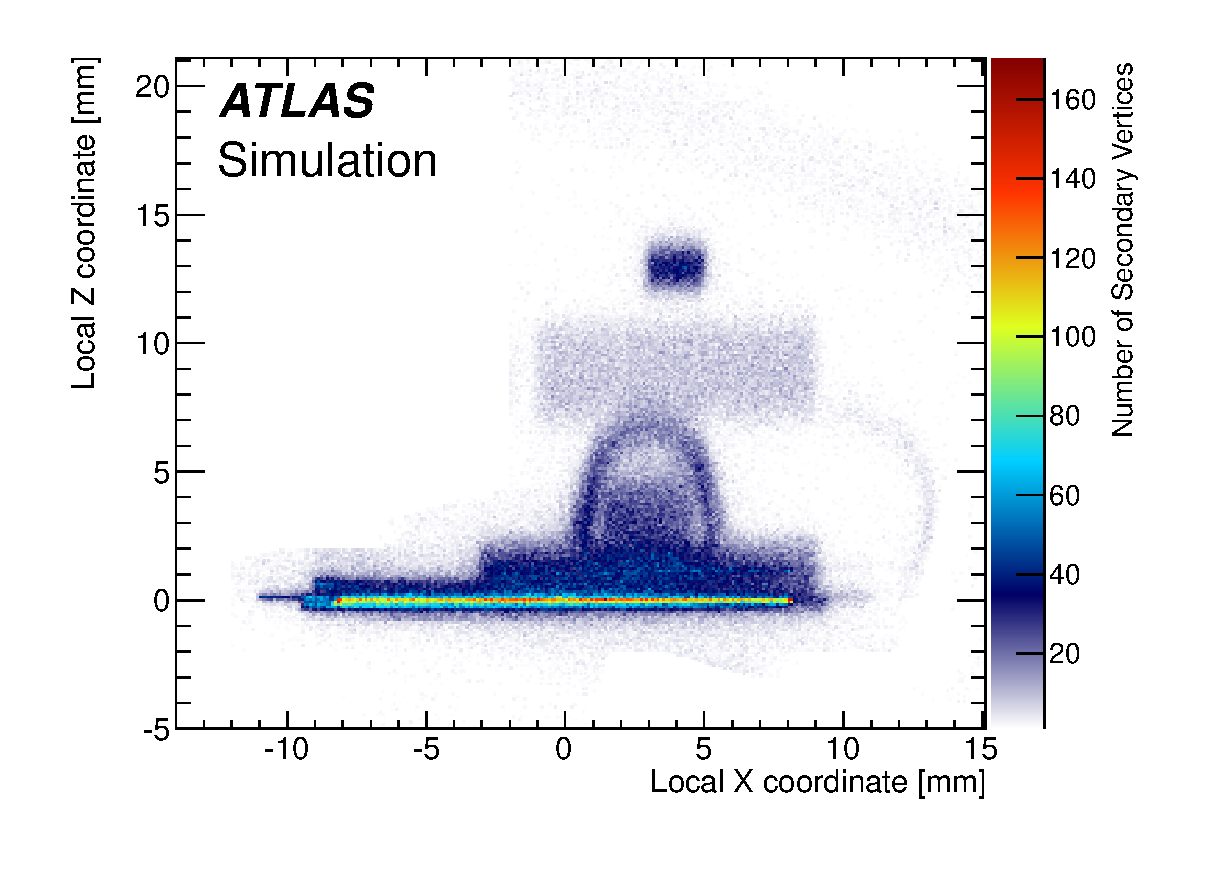
\includegraphics[width=.9\linewidth]{figures/theory/fig_10b.eps}
\caption{Number of secondary vertices in a module in the first layer of the pixel detector in data (top) and \ac{MC} (bottom). There are more events in the data than the \ac{MC} \cite{PERF-2015-06}.}
\label{fig:geant}
\end{figure}
\end{centering}

Custom \ac{ATLAS} code converts the energy deposited in active sensors into signals that resemble the expected detector response. These responses are typically very complicated with many parameters, and are frequently iterated on to best match the data. Electronic noise must also be added to correctly approximate the operating conditions of the detector. Additional alterations to this signal translation, including dead sensors and misalignments of the detector, can also be added at this stage. 

Once the simulated particles have been converted into detector signals, the same reconstruction software used on data can be used on the \ac{MC}, converting the detector signals back into particle interpretations. This reconstruction process is described in \autoref{ch:reconstruction}. The original information about the particles from the generator, referred to as \textit{truth} information, is also kept, and can be compared to the reconstruction output to study its efficacy.




 % ATLAS
% Chapter 4b
\chapter{Object Reconstruction in the ATLAS Detector} % Chapter title
\label{ch:reconstruction} 

Object reconstruction is the computation-intensive process of turning the signals from the approximately 100 million read-out channels of the ATLAS detector into a collection of particles and jets, the objects with which physics analysis can be performed. This process is complicated, and requires dedicated working groups in the ATLAS experiment that optimize the understanding of each type of object, which must all collaborate to provide a full picture of the events in the detector.

%---------------------------------------------------------------------------------------

\section{Electrons}
\label{sec:reco_electrons}

Electrons are identified through a combination of \ac{ID} and calorimeter measurements. They travel through the tracking system, leaving charge deposits in each layer, then are absorbed by the electromagnetic calorimeter. These two measurements work in conjunction to deliver high resolution measurements of electron momentum from low-\pt, where track curvature gives the most reliable measure of the electron's energy, to high-\pt, where the tracks are almost perfectly straight, but the calorimeter can still provide a reliable measurement. 

In the central region ($|\eta|<2.47$) of the ATLAS detector, electron reconstruction begins with the identification of energy deposits in the electromagnetic calorimeter. The calorimeter clusters are seeded by sliding longitudinal windows, which are measured in units of 0.025 in $\eta$ and $\phi$. 3$\times$5 unit windows are used, which require at least 2.5 \gev~in the window to form a seed \cite{Aad:2011mk}. 

These clusters are matched to \ac{ID} tracks by extrapolating the track to the middle layer of the calorimeter and identifying nearby clusters. If there are multiple tracks associated with a given cluster, tracks with silicon hits are preferentially chosen, and then the track with the smallest $\Delta R$ to the center of the cluster is selected. The track is used to determine the likely direction of bremsstrahlung radiation in the calorimeter, and maximum distance to match a track to a clusters expanded in the $\phi$ direction to account for this radiation.

The calorimeter clusters are then rebuilt in in larger windows, 3$\times$7 in the barrel and 5$\times$5 in the end-caps. An estimate of the energy is made by summing the measured calorimeter energy with estimates of the energy lost before the electron reached the calorimeter, energy outside of the cluster window, and energy not fully deposited in the calorimeter. These estimates are made with parametrized functions determined from a comparison of \ac{MC} and measurements taken by the presampler. 

The momentum is determined though a combination of the calorimeter and track measurements of the electron, while its $\eta$ and $\phi$ are taken from the track at its vertex. The energy of the electron is taken from the calorimeter cluster.

In the forward region, where no tracking is available, electron energy is determined more roughly. Calorimeter cells are formed into variable-sized clusters in regions of significant energy deposition, and the center of the cluster is used to determine angular coordinates of the electron. 

Electrons are identified using an algorithm that uses multivariate analysis to assign a likelihood that a candidate is a true electron based on input from just under twenty different variables. These include track quality, hadronic leakage, and cluster shape, incorporating information from as many subdetectors as possible in its determination of the candidate's quality. Each variable is assigned a \ac{PDF} for true electrons and background processes, and they are collectively used to provide a likelihood value which can be cut on. 

Three levels of identification, \texttt{LHLoose}, \texttt{LHMedium}, and \texttt{LHTight}, are defined with different likelihood cuts, with tighter cuts always a subset of the looser cuts. \autoref{fig:reco_el_eff} gives the efficiencies at each of these working points both for true electrons and for hadrons, which can be misidentified as electrons. Tighter working points have worse efficiencies, but lower misidentification rates. 

\begin{centering}
\begin{figure}[!hbt]
\myfloatalign
\includegraphics[width=.48\linewidth]{figures/reco/fig_01a.png}
\includegraphics[width=.48\linewidth]{figures/reco/fig_01a.png}
\caption{ Identification efficiencies from \ac{MC} samples for loose, medium, and tight working points. Left is the efficiency for identification of true electrons taken from $Z\rightarrow ee$ \ac{MC}, and right is the efficiency for mis-identification of jets as electrons taken from dijet \ac{MC} \cite{ATLAS-CONF-2016-024}.}
\label{fig:reco_el_eff}
\end{figure}
\end{centering}

\ac{MC} efficiencies can be compared to efficiencies measured in data using the tag-and-probe method, to obtain a \textit{scalefactor}, a correction factor applied to \ac{MC} to better emulate the rates at which electrons are reconstructed and identified. \autoref{fig:reco_el_sf} shows a comparison of the combined reconstruction and identification efficiencies in data and \ac{MC}, with the resulting scalefactors also displayed as the ratio. 

\begin{centering}
\begin{figure}[!hbt]
\myfloatalign
\includegraphics[width=.90\linewidth]{figures/reco/fig_14b.pdf}
\caption{ Combined electron reconstruction and identification efficiencies measured as a function of $\eta$ for data (using the tag-and-probe method on $Z\rightarrow ee$ events) and $Z\rightarrow ee$ \ac{MC}. Distributions include all electrons with \et > 15 \gev. \cite{ATLAS-CONF-2016-024}.}
\label{fig:reco_el_sf}
\end{figure}
\end{centering}

Electrons can also have \textit{isolation} requirements, cuts on nearby calorimeter activity or tracks. Isolation variables are primarily used to reject non-prompt leptons, which can be produced in heavy flavor hadron decays, converted photons, and misidentified hadrons. Cuts are made on the amount of nearby calorimetric energy and sum of the \pt of nearby tracks relative to the electron's energy, forming a series of working points. Fixed cut working points, which specify the relative fraction to cut on, can be used, but efficiency targeted working points are more popular. These include \texttt{Tight} and \texttt{Loose} working points, which operate at 95 and 98\% efficiency respectively, and working points that target tighter efficiencies at higher electron \pt, \texttt{Gradient} and \texttt{GradientLoose}. These working points each have 99\% efficiency for electrons with \pt > 60 \gev, but 90 and 95\% efficiencies at 25 \gev. 

\section{Photons}
\label{sec:reco_photons}

The reconstruction of photons is performed in parallel to electron reconstruction. Seed clustering is performed, and tracks are matched to these clusters, as in the case of the electron reconstruction described in \autoref{sec:reco_electrons}. 

Photons can be converted to electron-positron pairs in the \ac{ID}, leaving a pair of tracks, or they can pass through without conversion, leaving no tracks behind. As a consequence, calorimeter clusters resulting from photons can have no tracks associated with them, two tracks, or one track, in the case that one of the conversion tracks is not reconstructed. The reconstruction software attempts to identify all these scenarios and differentiate these processes from electron and hadron deposits \cite{1606.01813}.

Two-track clusters are required to consist of two oppositely charged tracks that emerge from a conversion vertex running parallel to one another. A likelihood that these are from electrons is determined using the high threshold hits in the \ac{TRT}, and cuts on this likelihood are made for tracks with and without silicon hits, 10 and 80\% respectively. The tracks are fit to produce the conversion vertex, and quality cuts are made, such as requiring that conversion vertices within the silicon volume correspond to tracks with silicon hits. 

Single track clusters occur most often from conversions in the outermost layers of the \ac{ID}, and are more difficult to reconstruct. Tracks are typically lost because the coverted electron is too low \pt to be reconstructed, or because the two tracks are so close together that they're identified as a single track. The single track is required to have at least a 95\% electron likelihood, and must not have a hit in the innermost layer of the pixel detector. The conversion vertex is defined as the first hit of the track. 

These conversion vertices are extrapolated to the calorimeter and matched to clusters. If multiple vertices are matched to a single cluster, preference is given to vertices with double tracks, silicon hits, and finally to tracks closest to the interaction point. 

Any cluster with neither a conversion vertex or a track reconstructed to it is identified as an unconverted photon. Clusters with conversion vertices are reconstructed as photons unless the cluster is also associated with an electron and the tracks associated with the cluster don't match the tracks associated with the conversion vertex. Single track clusters associated with electrons are instead identified as photons if the track has no silicon hits. 

The photon's energy is determined in 3$\times$5 (3$\times$7) windows for unconverted (converted) photons in the barrel, where the window is expanded to compensate for the increased spread of energy from the conversion products. In the endcap, the 5$\times$5 window is used in all cases. Like the electrons, the calibration of the photon's energy accounts for energy loss before the calorimeter, as well as energy deposited outside the cell and beyond the electromagnetic calorimeter.

Photon identification is performed in the range $|\eta|<2.37$ using a series of cuts on the shape of the shower in the electromagnetic calorimeter, as well as the amount of additional energy deposited in the hadronic calorimeter. Photons in the the so called \textit{crack} region of the calorimeter ($1.37<|\eta|<1.52$), where a discontinuity prevents accurate assessment of photon energy, are rejected. The identification has a \texttt{Loose} and a \texttt{Tight} working point. The \texttt{Tight} working point is used most often, and has an identification efficiency of 53–64\%(47–61\%) for unconverted (converted) photons with \et = 10 \gev~and 88–92\% (96–98\%) for photons with \et $\geq$ 100 \gev \cite{ATL-PHYS-PUB-2016-014}. Efficincies as a function of \pt measured in the 2016 data and compared to \ac{MC} can be seen in \autoref{fig:reco_photon_eff}.

\begin{centering}
\begin{figure}[!hbt]
\myfloatalign
\includegraphics[width=.48\linewidth]{figures/reco/photon_fig_01.pdf}
\includegraphics[width=.48\linewidth]{figures/reco/photon_fig_02.pdf}
\caption{ Comparison of tight identification efficiency measurements from data and $Z\rightarrow \ell\ell\gamma$ \ac{MC} for unconverted (left) and converted (right) photons, with an inclusive $\eta$ election. The bottom of each figure shows the ratio of data and \ac{MC} efficiencies. \cite{EGAM-2016-003}.}
\label{fig:reco_photon_eff}
\end{figure}
\end{centering}

Photon isolation, like electron isolation, can be determined as the combination of nearby calorimeter deposits and tracks. Fixed cuts on the isolation as a fraction of photon energy is typically used. A working point called \texttt{FixedCutTight} reconstructs the amount of calorimeter energy (excluding that of the photon) in a cone of $\Delta R  = 0.4$ around the photon and the amount of energy from the sum of track \pt in a cone of $\Delta R = 0.2$. Defined relative to the photon's \pt, this working point includes photons with calorimetric isolation less than 0.022\pt + 2.45 \gev~and track isolation less than 0.05\pt \cite{isolation}. 

\section{Muons}
\label{sec:reco_muons}

Muon reconstruction is performed independently in the \ac{ID} and the \ac{MS}, then the two measurements are combined when possible \cite{1603.05598}. The \ac{ID} reconstruction is performed using the tracking mechanism over the $|\eta|<2.5$ range. As with electrons, hits in the layers of the \ac{ID} are fit to tracks, a process described in more detail in \autoref{sec:NN}.

The \ac{MS} track reconstruction begins with a search in each muon chamber for patterns of hits consistent with a track, called \textit{segments}. The \ac{MDT} chamber hits are fit to a straight line, and nearby \ac{RPC} and \ac{TGC} chambers provide the coordinate orthogonal to the magnetic curvature for these hits. The \ac{CSC} segments are required to be loosely consistent with a track originating from the interaction point. 

These segments are then fit together, starting from the middle layers of the \ac{MS}, with track quality requirements on the resulting combinations based on the $\chi^2$ of the fits. Tracks must have at least two segments, except in the transition region between the barrel and endcap, where a single high quality segment can qualify as a track. Shared segments are allowed in the initial reconstruction, but after the combination, tracks with shared segments and low quality fits are removed.    

These \ac{MS} tracks are then combined with measurements from other parts of the ATLAS detector. The best quality muons are combined muons, which have \ac{ID} and \ac{MS} tracks associated to them, the hits of which are re-fit to form a combined track. \ac{MS} hits can be added or removed at this stage based on their consistency with the new track. Other types of muons exist, including extrapolated muons, which have only \ac{MS} tracks that are consistent with the interaction point, calorimeter-tagged muons, which combine an \ac{ID} track with a calorimeter deposit consistent with a muon, and segment-tagged muons, which combine an \ac{ID} track with a segment in the \ac{MS}. Muons with shared \ac{ID} tracks are not allowed, with preference given to combined muons, then calorimeter-tagged muons, and lastly segment-tagged muons. 

There are four muon identification working points for muons: \texttt{Loose}, \texttt{Medium}, \texttt{Tight}, and \texttt{High-p$_\texttt{T}$}. These working points all have different efficiencies for the identification of muons, balanced against the mis-identification of hadrons. One of the key variables for their discrimination is $q/p$ significance, which quantifies the consistency between the \ac{ID} and \ac{MS} measurements of momentum. The $\chi^2$ of the combined fit is also an important discriminator. 

The \texttt{Loose}, \texttt{Medium}, and \texttt{Tight} efficiencies are inclusive, with all \texttt{Tight} muons passing the \texttt{Medium} requirements, for example. The \texttt{Loose} requirement includes all types of muons, but allows muons without \ac{MS} tracks only in the $\eta<0.1$ range where coverage of the \ac{MS} is incomplete. The \texttt{Medium} working point includes only combined and extrapolated muons, and is the default for most ATLAS analyses. Extrapolated muons are allowed only in the $\eta$ range outside the \ac{ID} tracking system, a region often excluded by analyses because of the decreased quality. For the combined muons, at least three hits in at least two \ac{MDT} layers are required (except in the $\eta<0.1$ region) and a $q/p$ significance cut is made to reduce backgrounds. Even with the reduced requirements at low $\eta$, there is a drop in efficiency in this region, as shown in \autoref{fig:reco_muon_eta}. The \texttt{Tight} working point additionally cuts on $\chi^2$ and $p'$, another variable that quantifies the discrepancy between \ac{ID} and \ac{MS} \pt measurements. 

\begin{centering}
\begin{figure}[!hbt]
\myfloatalign
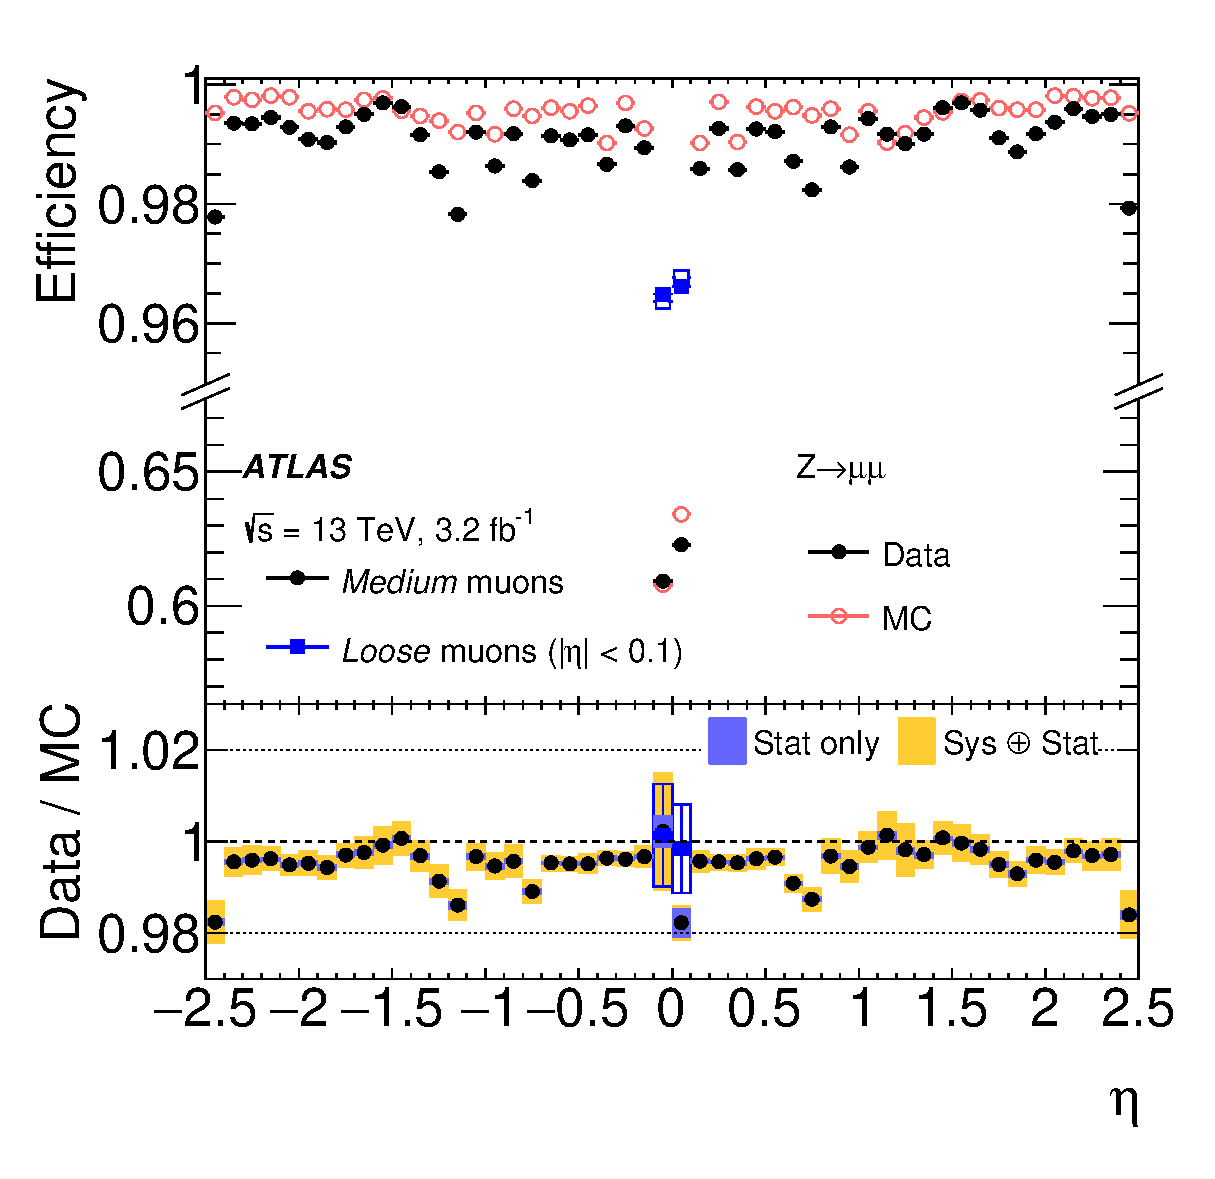
\includegraphics[width=.9\linewidth]{figures/reco/fig_03a.eps}
\caption{Muon reconstruction efficiency for the \texttt{Medium} working point measured with $Z\rightarrow\mu\mu$ events in data using the tag-and-probe method and in \ac{MC} as a function of $\eta$. The ratio between the two is shown at the bottom. \cite{1603.05598} }
\label{fig:reco_muon_eta}
\end{figure}
\end{centering}


The \texttt{High-p$_\texttt{T}$} working point is designed to maximize efficiency for high-\pt muons, at the cost of lower efficiencies for low-\pt muons. Muons must have at least three \ac{MDT} hits in three layers, which decreases efficiency but gives greatly improved \pt resolution. In addition, some regions of the \ac{MS} with low-performing chambers are vetoed to cut down on mismeasurement. Compared to the default working point these muons have much lower efficiency: 78\% (90\%) for \texttt{High-p$_\texttt{T}$} muons compared to 96\% (96\%) for \texttt{Medium} in the \pt range of 4-20 \gev~(20-100 \gev). The efficiency as a function of $\eta$ for this working point can be seen in \autoref{fig:reco_muon_eta_highpt}, where the efficiency loss due to the of vetoing of some chambers is especially apparent.

\begin{centering}
\begin{figure}[!hbt]
\myfloatalign
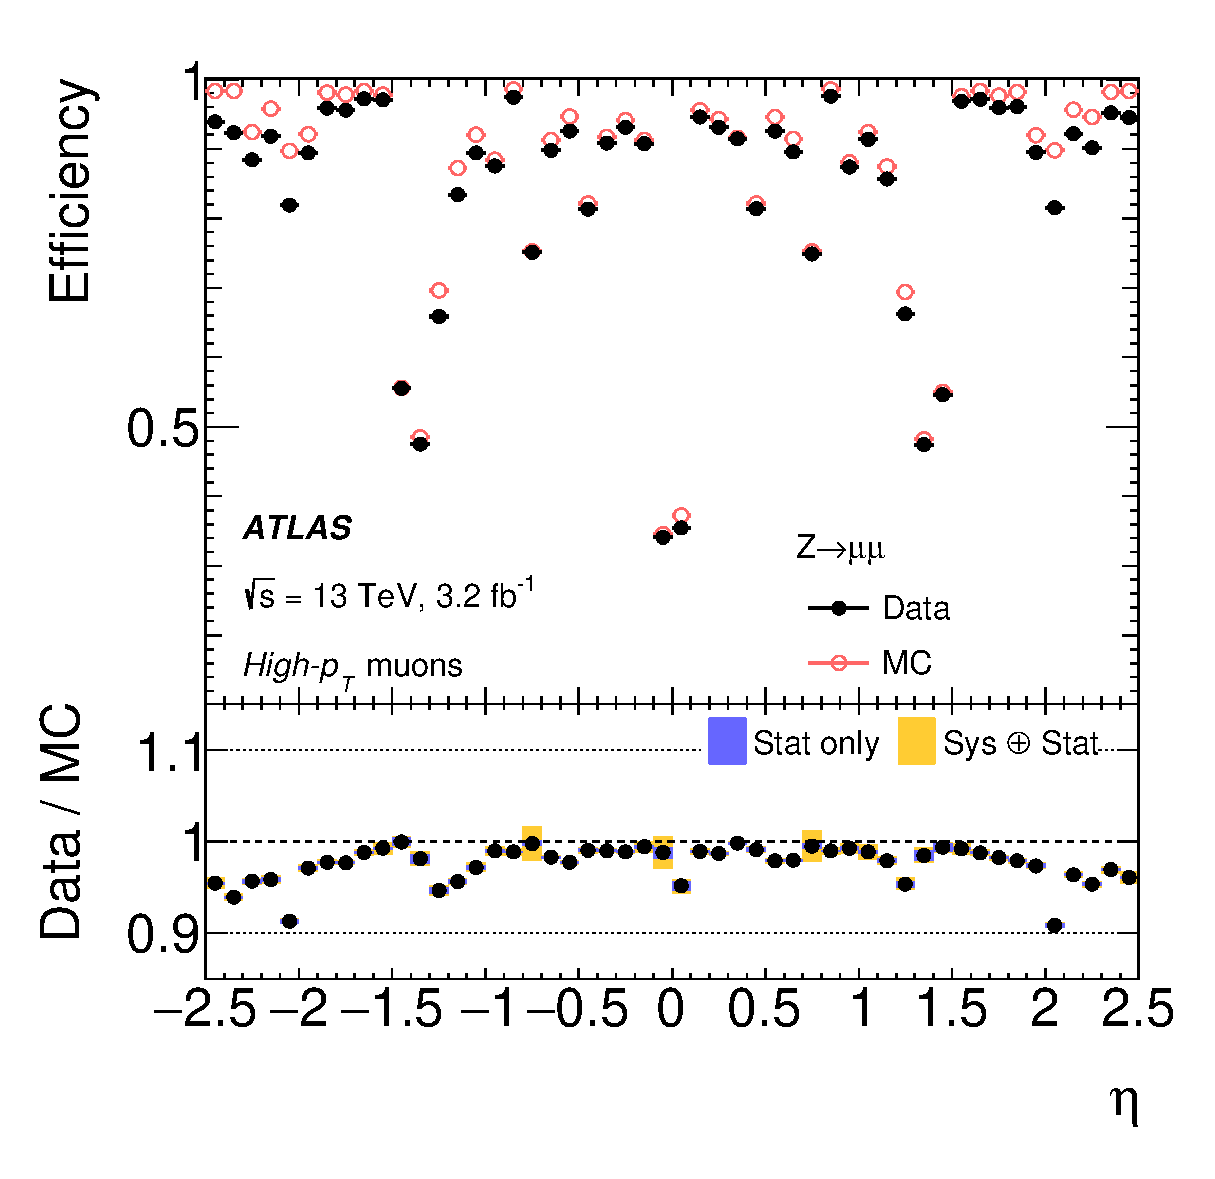
\includegraphics[width=.9\linewidth]{figures/reco/fig_03c.eps}
\caption{Muon reconstruction efficiency for the \texttt{High-p$_\texttt{T}$} working point measured with $Z\rightarrow\mu\mu$ events in data using the tag-and-probe method and in \ac{MC} as a function of $\eta$. The ratio between the two is shown at the bottom. \cite{1603.05598} }
\label{fig:reco_muon_eta_highpt}
\end{figure}
\end{centering}

The most common isolation selection for muons is designed in the same way as the electron isolation, and also called \texttt{GradientLoose}. It is constructed such that muons with \pt of 25 \gev~have an efficiency of 95\%, and muons with \pt of 60 \gev~have an efficiency of 99\%. 

\section{Jets}
\label{sec:reco_jets}

Jets are the most complicated objects to reconstruct in the ATLAS detector because each jet is an assembly of many hadronic particles. In contrast to a lepton, whose reconstructed energy can easily be compared to its true energy from simulation, even a jet's true energy is ambiguous, and is dependent on the choice of the jet's definition. The standard jet reconstruction algorithm used in the ATLAS experiment is called anti-$k_t$ \cite{Cacciari:2008gp}. 

This algorithm begins with calorimeter clusters defined by topologically connected cells with energy deposits significantly higher than the noise background. In fact, there are two collections of these clusters, one with cluster energies calibrated for electromagnetic showers (\acs{EM}), and another calibrated to hadronic showers. The second uses a method called \ac{LCW}, which first classifies a cluster as electromagnetic or hadronic based on the energy density and the shower depth, then applies a calibration according to the classification for each cluster.

The anti-$k_t$ algorithm is then applied to these clusters, which begins with the highest energy cluster and groups it with nearby clusters according to the distance measure

\begin{equation}
d_{ij} = min(k^{-2}_{ti}, k^{-2}_{tj}) \frac{\Delta_{ij}^2}{R^2}
\end{equation}

where $R$ is the algorithm's radius parameter, typically set to 0.4, $\Delta$ gives the angular separation of the two clusters, and $k_t$ is the transverse momentum associated with the cluster. Clusters are added to the jet within the cone radius, then the axis of the jet is reassessed. This process is repeated until a stable jet is produced. The inverse dependence on the $k_t$ of the cluster produces jets with energetic cores and softer edges, which matches the expectation from a hadronic shower. In addition it is infrared and collinear safe, with neither soft emission or collinear tracks altering the reconstruction of the jet. 

A series of calibrations are then applied to these jets. The first is to correct for additional hadronic energy due to pile-up, shown in \autoref{fig:reco_jet_nvtx}. To do this, a correction taken from \ac{MC} and parametrized in terms \pt and $\eta$, as well as the number of primary vertices in the event as well as the average number of vertices, which makes correction for out-of-time pile-up possible. Next, jets are corrected to have their origin at the primary vertex instead of the center of the ATLAS detector. After that, the jets are corrected based on jet energy and $\eta$ dependent \ac{JES} factors derived from \ac{MC}. \autoref{fig:reco_JES} shows the energy response, the inverse of these factors, for \ac{EM} jets. Lastly, some regions of the detector have been shown to have a bias in $\eta$ measurement of jets, and this is accounted for. 

\begin{centering}
\begin{figure}[!hbt]
\myfloatalign
\includegraphics[width=.9\linewidth]{figures/reco/fig_02.pdf}
\caption{ Distribution of event \pt density, $\rho$, taken from \ac{MC} dijets for different numbers of primary vertices. \cite{ATL-PHYS-PUB-2015-015} }
\label{fig:reco_jet_nvtx}
\end{figure}
\end{centering}

\begin{centering}
\begin{figure}[!hbt]
\myfloatalign
\includegraphics[width=.9\linewidth]{figures/reco/fig_04a.pdf}
\caption{ Energy response as a function of energy and $\eta$ for \ac{EM} jets in dijet \ac{MC}. \cite{ATL-PHYS-PUB-2015-015} }
\label{fig:reco_JES}
\end{figure}
\end{centering}

In addition to correcting for additional energy due to pile-up, it is necessary to reject reconstructed jets that come from pile-up vertices. To accomplish this, a multivariate alogrithm called \ac{JVT} was created which builds upon an older method, \ac{JVF} \cite{ATLAS-CONF-2014-018}. The original method vetoed jets by summing the total \pt of associated tracks and assessing the fraction of that \pt that came from tracks associates with the event's primary vertex. This fraction decreases with higher pile-up, making the construction of an explicit cut difficult in pile-up varying conditions. \ac{JVT} improved on the method by producing a pile-up corrected \ac{JVF} variable and including it in the inputs of the tagger with other variables including a similar variable, where the sum of track \pt is replaced with the calibrated jet \pt. \autoref{fig:reco_jvt} shows the efficiency and fake rate for the two methods, demonstrating \ac{JVT}'s superior ability to reject pile-up jets even in events with many pile-up vertices.

\begin{centering}
\begin{figure}[!hbt]
\myfloatalign
\includegraphics[width=.48\linewidth]{figures/reco/jvt_fig_06b.eps}
\includegraphics[width=.48\linewidth]{figures/reco/jvt_fig_07a.eps}
\caption{ Dijet \ac{MC} distributions of the number of pile-up jets passing the \ac{JVT} and \ac{JVF} cuts (left) and the efficiency for jets from the primary vertex (right) as a function of number of primary vertices in the event \cite{ATLAS-CONF-2014-018}. }
\label{fig:reco_jvt}
\end{figure}
\end{centering}

It is possible to differentiate jets resulting from $b$-hadron decays from other jets due to the non-negligible lifetimes of the hadrons. Many \ac{BSM} processes preferentially produce $b$ quarks, as does any process involving top quarks, so this identification can be very useful for targeting specific decays in many analyses. Multivariate techniques are used to identify secondary vertices using the \ac{ID}\cite{ATL-PHYS-PUB-2015-022}. In ATLAS, separate algorithms are used to identify jets with tracks with significantly non-zero impact parameters, tracks that reconstruct a secondary vertex, and tracks that can be identified with a chain of vertices beginning with the primary vertex. This information is fed into a boosted decision tree called \texttt{MV2c20}, which outputs a discriminant shown in \autoref{fig:reco_mv2}. Using this discriminant, a working point is chosen such that $b$-jets can be identified with a 70\% efficiency, with mis-identification rates at around 12\% for $c$-jets and 0.2\% for light-flavor jets.

\begin{centering}
\begin{figure}[!hbt]
\myfloatalign
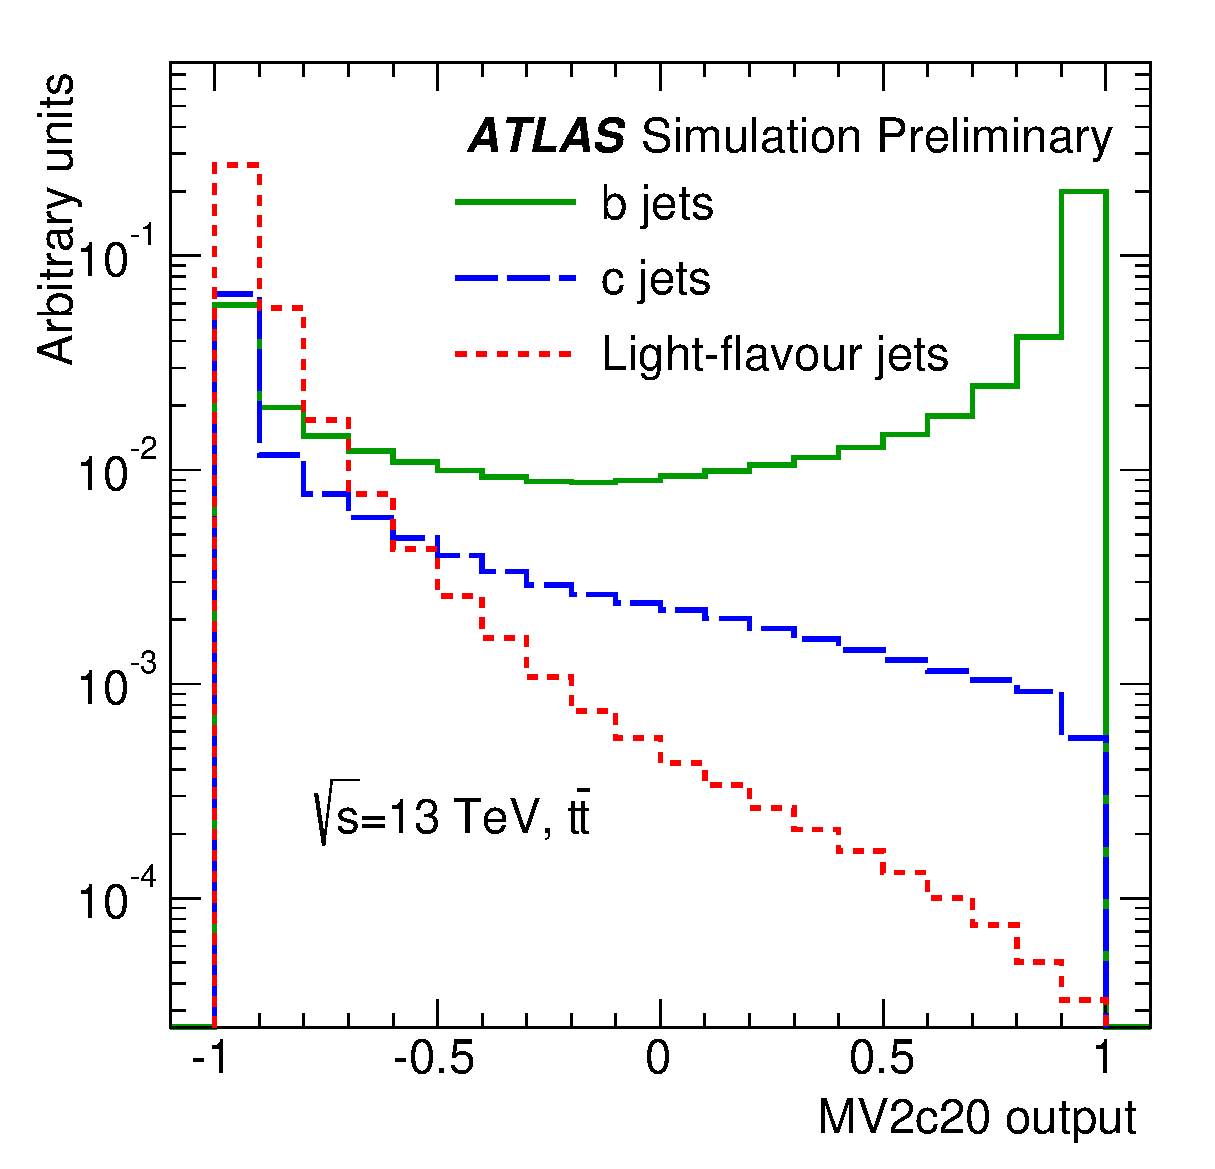
\includegraphics[width=.9\linewidth]{figures/reco/fig_08.eps}
\caption{ Distribution of \texttt{MV2c20} output for $b$-jets, $c$-jets, and light-flavor jets \cite{ATL-PHYS-PUB-2015-022}. }
\label{fig:reco_mv2}
\end{figure}
\end{centering}

\section{Overlap Removal}
\label{sec:reco_or}

Because most of these reconstruction methods are run independently, it is common for energy deposits and tracks to be shared between multiple particles of different types. To account for this, a process called \acf{OR} is used, which iteratively removes overlapping objects. The process is performed at the \textit{baseline} level, a set of loose selections on objects which are later further refined to create the \textit{signal} objects used in analysis.

The first step in the \ac{OR} process is to remove reconstructed jets that appear to be due to calorimetric deposits from an electron. To accomplish this, any baseline jet within $\Delta R = 0.2$ from a baseline electron is removed. A caveat is added due to the frequent production of leptons in the decay of heavy-flavor jets; if the jet is $b$-tagged, the electron will be removed instead. After these electrons and jets have been removed, a new search is done for jets and electrons within $\Delta R = 0.4$ of one another. In this iteration, the electron is removed, again to reduce backgrounds from heavy-flavor decays.

Next, the muon-jet \ac{OR} is applied, which is very similar to that of the electron. Any jet within $\Delta R = 0.2$ of a muon is removed, unless the jet is $b$-tagged, in which case the muon is removed due to the likelihood that it resulted due to a heavy-flavor decay. The muon-jet \ac{OR} then differs from the electron's in that a \pt-based $\Delta R$ cut is used in the last step. Muons within $\Delta R < min(0.04 + (10 \gev)/\pt, 0.4)$ of a jet are removed, with the shrinking cone for high-\pt muons designed to improve efficiency for energetic muons that produce significant calorimeter deposits, while still rejecting the heavy-flavor muons that are typically lower \pt. 

The last step is to remove electrons resulting from muon bremsstrahlung. Any remaining electron within $\Delta R = 0.1$ of a muon is removed from the event. 

In addition, in the case that photons are reconstructed\footnote{As described in \autoref{ch:objects}, the default configuration of this analysis does not include the reconstruction of photons, however, for certain background estimations that require photons, an alternate reconstruction including photons is performed.}, photon-electron \ac{OR} and photon-jet \ac{OR} are performed. Baseline photons within $\Delta R = 0.4$ of an electron are removed, as are jets within $\Delta R = 0.4$ of a remaining photon.

\section{Missing Transverse Energy}
\label{sec:reco_met}

Missing transverse energy, \met, is the negative vector sum of \pt of the objects in an event. Because colliding particles have no initial transverse momentum, the true value of this quantity should be zero unless a particle escapes the detector without being measured, as neutrinos do. In practice, the reconstructed \met can also be non-zero due to mismeasurement. \met reconstruction is perhaps the most complex because it depends on all other object reconstructions performed in the ATLAS detector. 

\met components are calculated independently for each type of baseline object reconstructed, as well as for a soft term, which accounts for low-\pt radiation from the primary vertex \cite{ATL-PHYS-PUB-2015-023}. This component comprises all \pt observed by the ATLAS detector but not associated with a baseline object, and can be calculated based either based on calorimeter or track measurements. While the \ac{CST} is very sensitive to pile-up, the \ac{TST} is much more robust, as it can exclude tracks emanating from pile-up vertices. Tracks associated with any reconstructed object are also removed. \autoref{fig:reco_met_tst} shows the \ac{TST} resolution's dependence on number of primary vertices, which is considerably more stable than \ac{CST}.

\begin{centering}
\begin{figure}[!hbt]
\myfloatalign
\includegraphics[width=.9\linewidth]{figures/reco/met_fig_04b.eps}
\caption{ Distributions of the resolution of the $x$ and $y$ components of \ac{TST} \met in $Z\rightarrow\mu\mu$ events in data and \ac{MC} \cite{ATL-PHYS-PUB-2015-027}. }
\label{fig:reco_met_tst}
\end{figure}
\end{centering}

\autoref{fig:reco_met_terms} shows the the \met resulting from muons, jets, and the soft term in $Z\rightarrow\mu\mu$ events. These events very rarely have any true \met, so these distributions primarily demonstrate how mismeasurement of various objects contributes to the \met term. The jet and muon distributions both have significant high tails, while the soft term falls off much more quickly. 

\begin{centering}
\begin{figure}[!hbt]
\myfloatalign
\includegraphics[width=.9\linewidth]{figures/reco/met_fig_02a.eps}
\includegraphics[width=.9\linewidth]{figures/reco/met_fig_02b.eps}
\includegraphics[width=.9\linewidth]{figures/reco/met_fig_02c.eps}
\caption{ Distributions of the jet term (top left), muon term (top right), and \ac{TST} (bottom) \met in $Z\rightarrow\mu\mu$ events in data and \ac{MC} \cite{ATL-PHYS-PUB-2015-027}. }
\label{fig:reco_met_terms}
\end{figure}
\end{centering}




 % Reconstruction
% Chapter 3

\chapter{Application of a Neural Network to Pixel Clustering} % Chapter title

\label{sec:NN} % For referencing the chapter elsewhere, use \autoref{ch:mathtest}

%----------------------------------------------------------------------------------------

%----------------------------------------------------------------------------------------

\section{Clustering in the Pixel Detector}

Creating tracks from individual hits in the Inner Detector is one of most computationally challenging parts of the reconstruction of \ac{ATLAS} events. Each event typically contains thousands of hits in the pixel detector alone, which must be combined into one coherent picture of which particles traversed the detector, and how they moved and lost energy as they traveled. A typical particle deposits charge in several pixels per layer, forming a series of clusters which can be connected together to form a track. This track can in turn be used to measure the charge, momentum, and trajectory of the particle. 


\begin{centering}
\begin{figure}[bth]
\myfloatalign
\includegraphics[width=.90\linewidth]{figures/nn/cluster_types.pdf}
\caption{A few possible types of clusters in the Pixel Detector. $(a)$ shows a single particle passing through a layer of the detector, $(b)$ shows two particles passing through the detector, creating a single merged cluster, and $(b)$ shows a single particle emitting a $\delta$-ray as it passes through the detector \cite{PERF-2012-05}.}
\label{fig:cluster_types}
\end{figure}
\end{centering}

The process of going from clusters to track is relatively simple in an isolated environment in which one particle travels cleanly through all the layers, but can be complicated by multiple close-by tracks and by a single particle's emission of low energy particles, called $\delta$-rays. In these cases, it can be hard to tell how many particles were involved in creating a cluster, and where exactly each of those particles passed through the layer. A few examples of particle interactions with the pixel sensor can be seen in \autoref{fig:cluster_types}. 

Clusters are initially made by a process called \acf{CCA}. In this process, pixels in a given layer are grouped together if they share any edge or corner. The position of the resulting cluster is defined by local $x$ and $y$ coordinates, which describe its position and size within the pixel module on which it appears. Determining the position of the particle that formed that cluster is less straightforward, and has recently been updated from a charge interpolation method to a method using a \ac{NN}. 

\subsection{Charge Interpolation Method}

A typical cluster contains a few pixel hits spanning in the $x$ and $y$ directions, each with its own measurement of charge deposition, or \ac{ToT}. In the charge interpolation method, these individual hits are combined to make one estimation of the position a single particle which passed through them, using the following equation: 

\begin{eqnarray}
x_{cluster} = x_{center} + \Delta_x(\phi,N_{row}) \cdot \left[ \Omega_x -\frac{1}{2} \right] \\
\label{eq:analogx}
x_{cluster} = x_{center} + \Delta_x(\phi,N_{row}) \cdot \left[ \Omega_x -\frac{1}{2} \right]
\label{eq:analogy}
\end{eqnarray}

where $\Omega_{x(y)}$ is defined by

\begin{equation}
\Omega_{x(y)} = \frac{q_{last~row(col)}}{q_{first~row(col)} + q_{last~row(col)}}
\end{equation}

and $q$ represents the \ac{ToT} of a given pixel, and $\Delta_{x(y)}$ is a function derived from either data or \ac{MC} and produces an output related to the projected length of the particles track on the pixel sensor and is measured as a function of $\phi$, the incident angle of a particle on the sensor, and $N_{row(col)}$, the number of pixels in the $x$ and $y$ direction. 

In a simple case, such as $(a)$ of \autoref{fig:cluster_types} , this method works quite effectively. However, in cases like $(b)$, it has no ability distinguish two-particle from one-particle clusters, and can only assign a cluster center between the two particles' locations, despite that intermediate pixel having the lowest \ac{ToT}. Furthermore, because this method can't differentiate two-particle clusters, the tracking software can't use that information to preferentially allow multiple tracks to share two-particle clusters. Allowing tracks to share clusters indiscriminately in dense track environments creates fake tracks from the many possible cluster combinations, so this cannot be broadly permitted. In cases like $(c)$, the $\delta$-ray will bias the measurement of the particle's position in whichever direction it is emitted. 

\subsection{Improving Measurement with Neural Networks}

To address these problems, a series of \acp{NN} were created \cite{PERF-2012-05}. The first estimates the number of particles in a given cluster, the second estimates their positions within the cluster, and the third assesses the uncertainty of the position measurement. They are referred to, respectively, as the ``Number'', ``Position'', and ``Error'' \acp{NN}.

These \acp{NN} are taken from the AGILE\textit{Pack} library \cite{agile}, and trained using simulated \ac{ATLAS} \ac{MC}. Each \ac{NN} is given the following inputs: 
\begin{itemize}
\item a $7\times7$ grid of cluster \ac{ToT} information\footnote{Clusters spanning more than seven pixels in either direction are rare, but when they occur they are rejected, and the original charge interpolation estimate of a single particle's position is kept.}
\item a 7-element vector containing the $y$-size of the pixels in the grid\footnote{The pixel detector contains some long pixels at the edges of modules, and this is intended to help the \ac{NN} identify these cases.}
\item the layer of the pixel detector that the cluster was observed in
\item a variable indicating whether the cluster is located in the barrel or endcap
\item $\theta$ and $\phi$ variables projecting the incident angles of the particle on the sensor\footnote{If the \ac{NN} is applied before tracking is performed, these angles project to the nominal interaction point, and if tracking has already been performed, the angles are taken from the track fit to the cluster.}
\item the pixel module's $\eta$ index, a label assigned to each module that differentiates modules based on their $\eta$ position
\end{itemize}

After the Number \ac{NN} predicts a number of particles associated with the cluster, required to be between 1 and 3, the same inputs are fed to one of three Position \acp{NN} based on the determined number of particles, which then outputs the $x$ and $y$ positions of each of the particles. Then, the same inputs combined with the output of the Position \ac{NN} are fed into one of three Error \acp{NN} (also distinguished by number of particles), which outputs an uncertainty for each of the position predictions made. An example of the output of this process can be seen in \autoref{fig:merged_cluster}, where the improved position resolution from the ability to identify a multi-particle cluster is evident. 

\begin{centering}
\begin{figure}[bth]
\myfloatalign
\includegraphics[width=.90\linewidth]{figures/nn/merged_cluster.png}
\caption{One example of a two-particle cluster and its truth information compared with the output of the \acp{NN}. The boxes represent pixels, with a color scale indicating \ac{ToT}. At top, the $p(N=i)$ values give the output of the Number \ac{NN}, the probabilities that the cluster contains 1, 2, and 3 particles. Given the highest probability is for $N=2$, the other \acp{NN} predict the postion and errors of the two particles (in white). The black arrows and squares represent the truth information from the cluster, and the black dot and dotted line show the position measurement for the un-split cluster \cite{PERF-2012-05}.}
\label{fig:merged_cluster}
\end{figure}
\end{centering}

The particle location predictions from the \acp{NN} are then handed to the tracking software, which now can use these multiple particle position estimations as independent hits to be fit. As a result, tracks in dense environments have fewer clusters shared between multiple tracks, and their trajectories are known to a greater degree of precision. 


\section{Impact of the Neural Network}

The \ac{NN} was first applied to 7 \tev~data, where it improved position resolution for particles in small and large clusters. \autoref{fig:7tev_res} shows the improvement from the addition of the \ac{NN} in $x$ resolution in different cluster sizes. The improvement from charge interpolation clustering is particularly evident in the 4-pixel case, where the double peaked structure of the interpolation method has been completely removed with the \ac{NN}.  

\begin{centering}
\begin{figure}[!htb]
\myfloatalign
\includegraphics[width=.9\linewidth]{figures/nn/3x_res.pdf}
\includegraphics[width=.9\linewidth]{figures/nn/4x_res.pdf}
\caption{$x$ resolutions for clusters with 3 (top) and 4 (bottom) pixels in the $x$ direction in 7 \tev data for \ac{CCA} (using only charge interpolation to determine position) and \ac{NN} clustering taken from \ac{MC} \cite{PERF-2012-05}.}
\label{fig:7tev_res}
\end{figure}
\end{centering}

\subsection{The Neural Network in 13 TeV Data}

In Run 2, the tracking algorithm is first run on the \ac{CCA} clusters with positions determined via charge interpolation, where it constructs tracks with loose quality requirements. In this step, the tracking algorithm allows shared clusters, clusters used in multiple track fits \cite{ATL-PHYS-PUB-2015-044}. The \ac{NN} is then used to identify which clusters are likely to have had multiple particles pass through them, and to estimate the positions of those particles. In the case that the cluster is determined to have resulted only from one particle, tracks that share that cluster are penalized. In general, tracks with more than two shared clusters are rejected.

Because the \ac{NN} is trained only with \ac{MC} simulations, any mismodeling of the way charge is deposited in the \ac{ATLAS} detector could cause the \ac{NN} to perform in an unexpected way when applied to data. The potential impact of this mismodeling was investigated with 13 \tev~\ac{MC} \cite{ATL-PHYS-PUB-2015-052}. The goal of these studies was to determine which variables the \ac{NN}'s predictions were most sensitive to, and whether it was likely that these variables could be mismodeled enough to produce unexpected results in data. 

One example of a variable capable of significantly altering the \ac{NN} outputs was the overall charge scale. To study its impact, the \ac{ToT} of all pixels in a cluster were scaled up and down, and the resulting outputs of the \ac{NN} were compared, as shown in \autoref{fig:13tev_charge_robustness}. In this case, the likelihood to misidentify multi-particle clusters and single particle clusters depended significantly on this scaling. However, experts on the simulation of this scale agree that it's unlikely to be mismodeled by more than 10\%, so very extreme effects from a difference between data and \ac{MC} are unlikely. Overall, it was found that variations on the cluster charge produced a significant impact on predictions, while all other variations, such as incidence angle variation and spatial smearing of charge, had a minimal effect. 

\begin{centering}
\begin{figure}[bth]
\myfloatalign
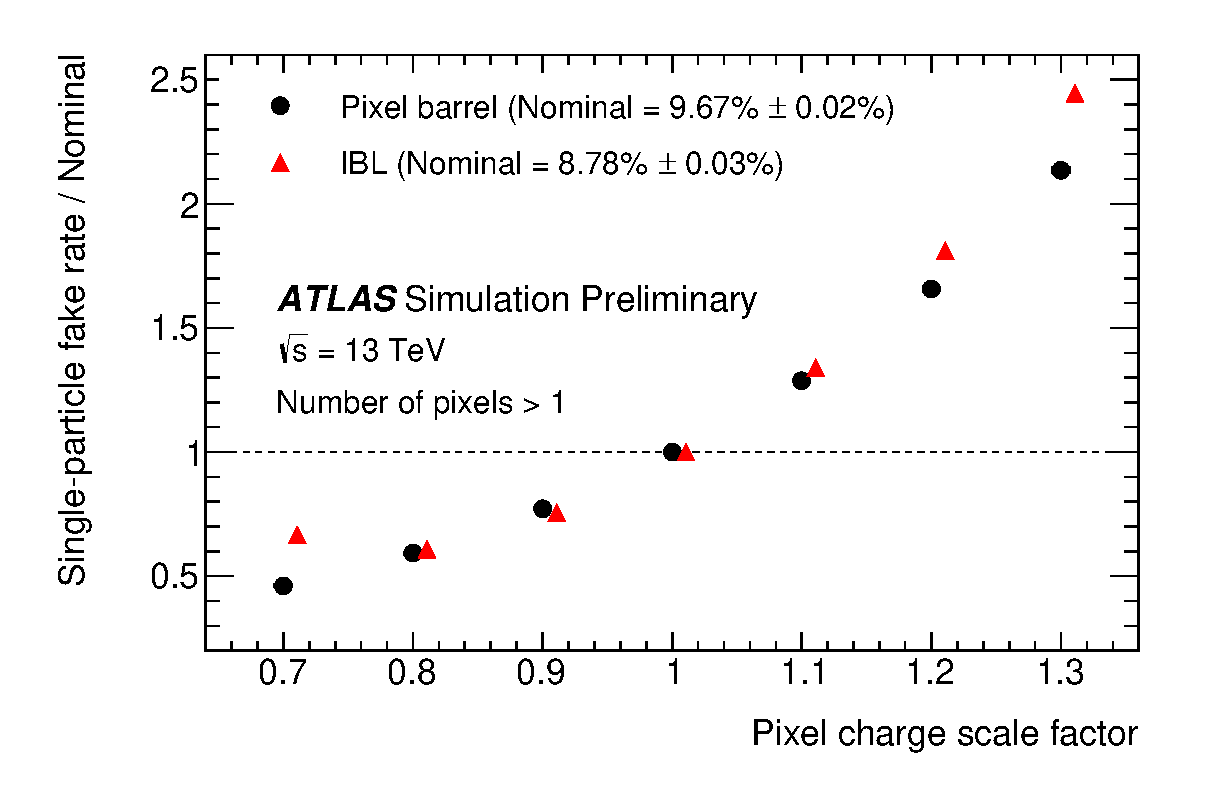
\includegraphics[width=.9\linewidth]{figures/nn/fig_05a.eps}
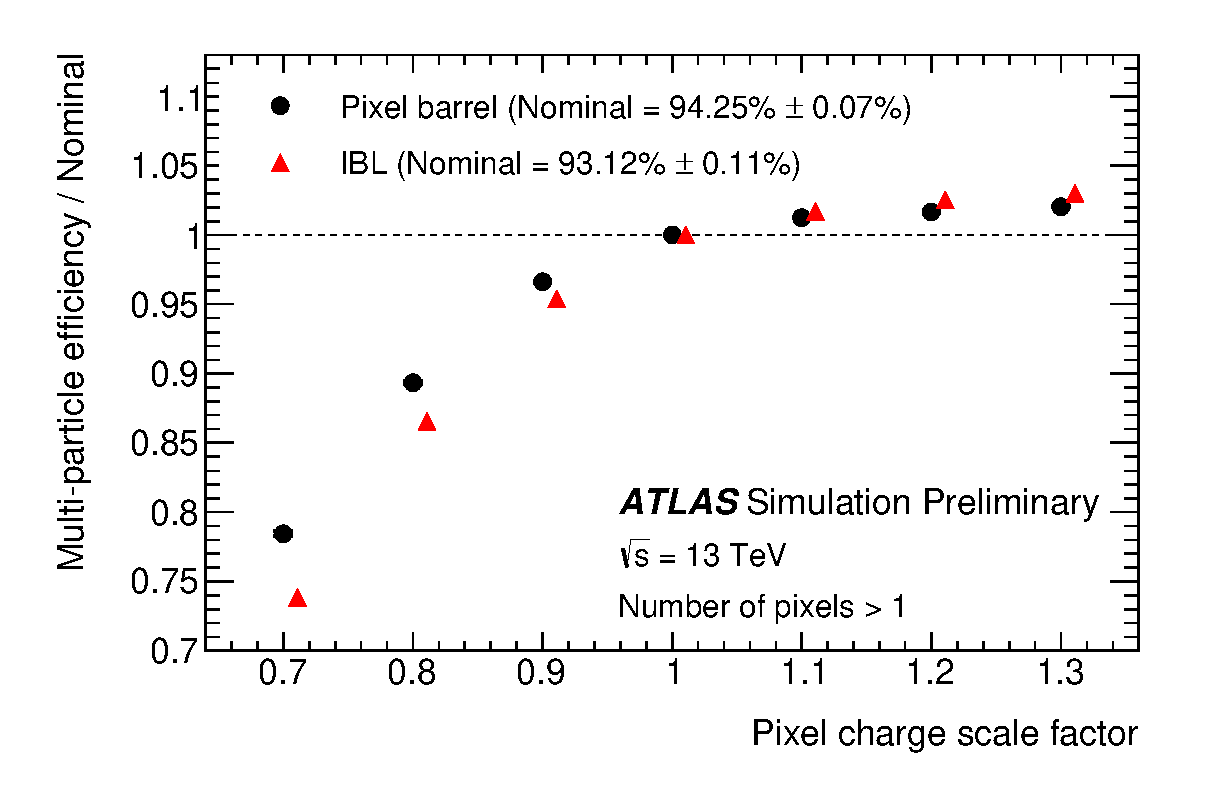
\includegraphics[width=.9\linewidth]{figures/nn/fig_05b.eps}
\caption{Performance of the pixel neural network used to identify clusters created by multiple charged particles, as a function of constant coherent scaling of the charge in each pixel in the cluster. The top figure shows the rate at which the neural network wrongly identifies clusters with one generated particle as clusters with multiple particles. The bottom figure shows the rate at which the neural network correctly identifies clusters generated by multiple particles as such.}
\label{fig:13tev_charge_robustness}
\end{figure}
\end{centering}

In addition to studies on the impact of alterations of individual simulation variables, studies directly comparing the \ac{NN} output in data and \ac{MC} were performed. \autoref{fig:13tev_fractions} shows a comparison of how often the \ac{NN} identifies different types of clusters in data and \ac{MC}. Each figure is made using by selecting pairs of collimated tracks that share a common cluster on a given layer, then calculating the fraction of those clusters that are determined by the \ac{NN} to be single or multi-particle clusters. This fraction is plotted as a function of the distance between the two tracks in the cluster's layer. Very good agreement is seen between the two samples, demonstrating that the \ac{MC}-trained \ac{NN} performs similarly on both \ac{MC} and data.

\begin{centering}
\begin{figure}[!htb]
\myfloatalign
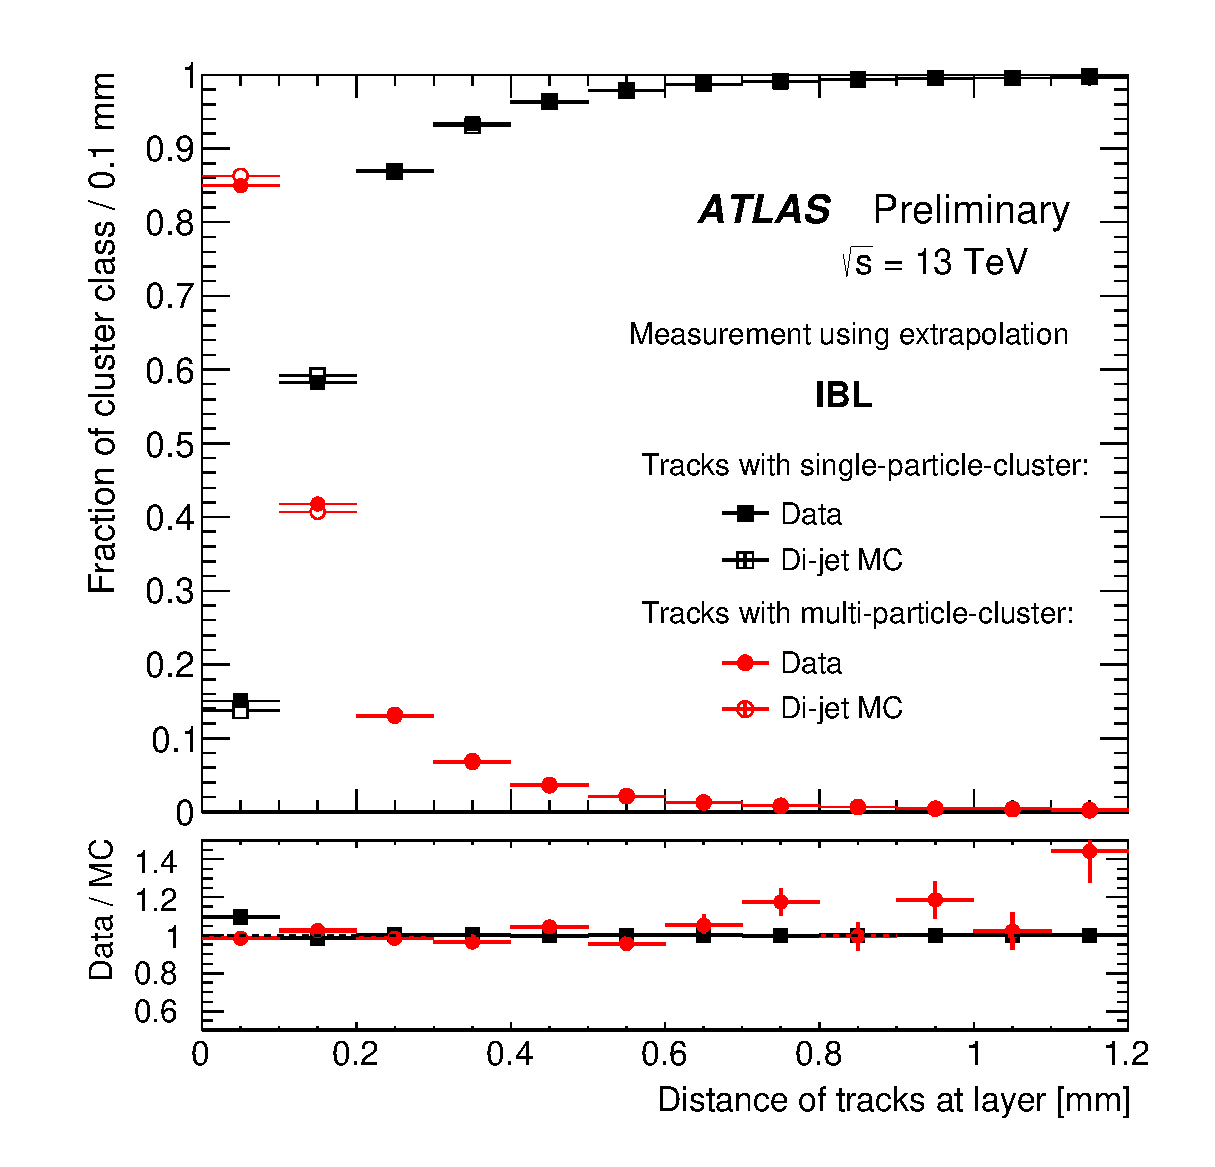
\includegraphics[width=.9\linewidth]{figures/nn/fig_07a.eps}
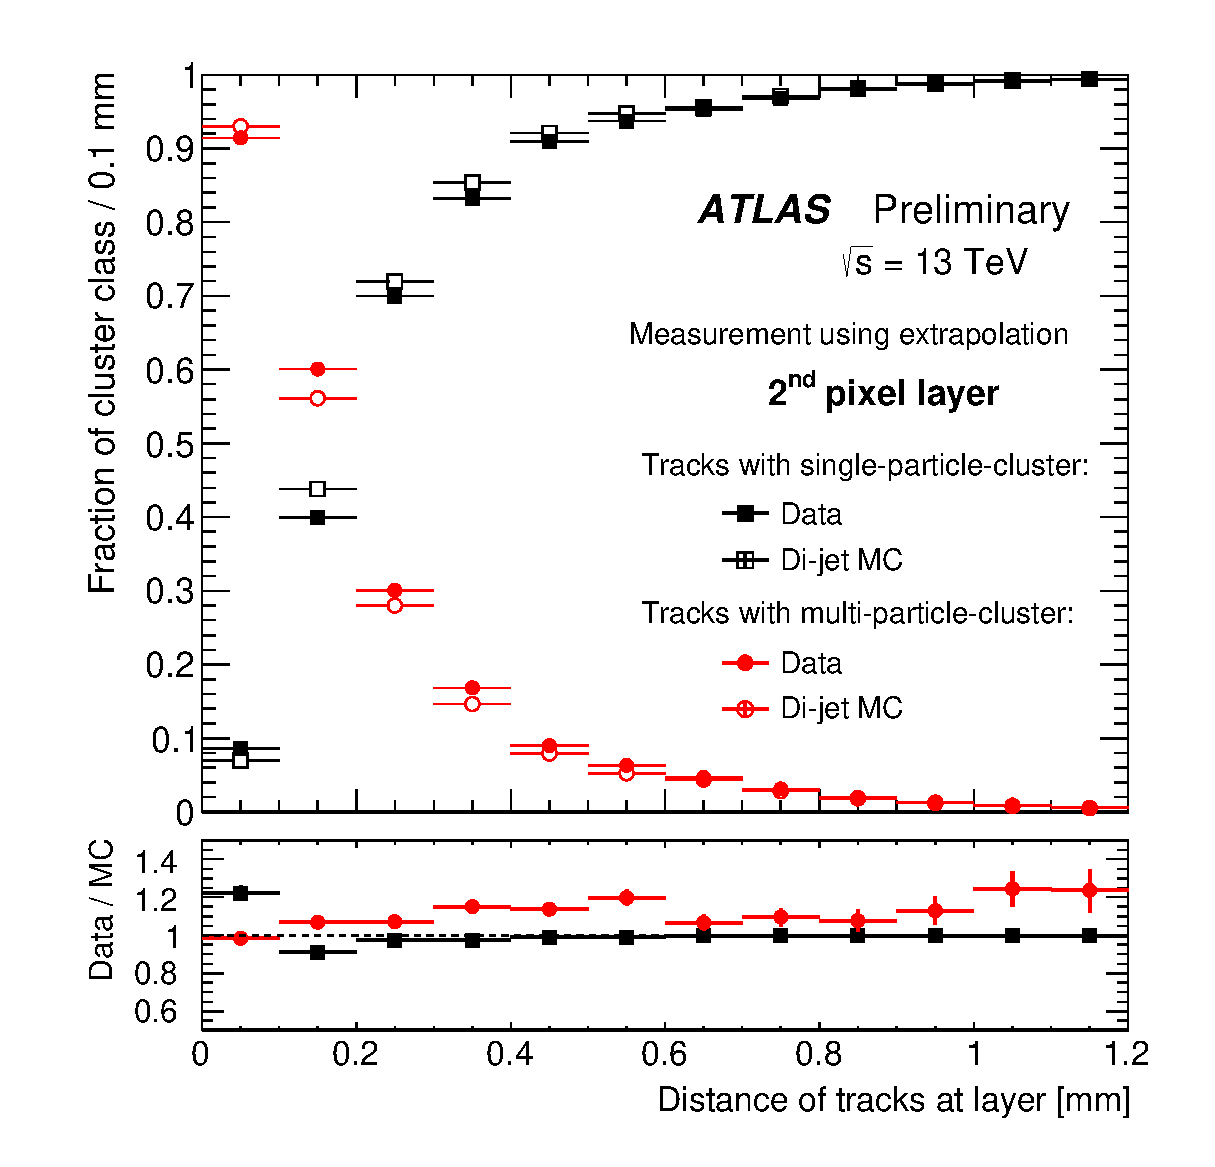
\includegraphics[width=.9\linewidth]{figures/nn/fig_07b.eps}
\caption{Fraction of cluster classes as a function of the distance between tracks for IBL (top) and 2nd pixel layer (bottom).}
\label{fig:13tev_fractions}
\end{figure}
\end{centering}



 % NN

\cleardoublepage % Empty page before the start of the next part

%------------------------------------------------

\ctparttext{This section describes an analysis of the ATLAS data carried out by the author and her analysis team. The analysis was performed on events from $p-p$ collisions provided by the \ac{LHC} at $\sqrt{s}$=13 TeV. It searches for events like those described in \autoref{sec:simplified_models}, which contain a Z boson decaying to leptons, jets, and missing transverse energy. The selection of a signal region in which to search for these events, background estimates, systematic uncertainty estimates, results, and interpretations are all discussed.} % Text on the Part 2 page describing the content in Part 2

\part{Searching for Supersymmetry} % Second part of the thesis
\label{part:search}

% Chapter 7

\chapter{Background Processes} % Chapter title

\label{ch:background_processes} 

%----------------------------------------------------------------------------------------

This analysis is fundamentally a search for \ac{SUSY} in events with two leptons whose invariant mass is consistent with a $Z$ boson. Additional event selections are made to reduce \ac{SM} processes relative to potential \ac{SUSY} processes, defined by simplified models discussed in \autoref{sec:simplified_models}. These models include the production of strongly-charged, high-mass particles, which results in events with jets and high \HT, the scalar sum of the \pt of all jets and the two leading leptons in the event. These $R$-parity conserving \ac{SUSY} models also produce decay chains that terminate with a stable, electrically neutral particle, which produces \MET when it passes through \ac{ATLAS} without detection. All of these features can help isolate these events from backgrounds. To understand what cuts would optimize the sensitivity of the search, it is essential to first understand what these \ac{SM} backgrounds are. 

\begin{centering}
\begin{figure}[bth]
\myfloatalign
\includegraphics[width=.70\linewidth]{feynman/ttbar.pdf}
\caption{An example Feynman diagram of \ttbar production and decay.}
\label{fig:ttbar}
\end{figure}
\end{centering}

\paragraph{Top-antitop (\ttbar)} production is the largest background for this search. \autoref{fig:ttbar} shows an example of this process, which results in two jets, leptons, and neutrinos, which are seen in the detector as \MET. Thus, \ttbar events naturally have high \MET and \HT, jets, and leptons from two different $W$ boson decays, which may coincidentally form an invariant mass consistent with a $Z$ boson. These events are very difficult to separate from potential signals, though keeping the mass window small and requiring \MET and \HT above the typical values for \ttbar events helps reduce this background.

\begin{centering}
\begin{figure}[bth]
\myfloatalign
\includegraphics[width=.70\linewidth]{feynman/diboson.pdf}
\caption{An example Feynman diagram of the production and decay of a WZ event.}
\label{fig:diboson}
\end{figure}
\end{centering}

\paragraph{diboson ($VV$)} production is the next leading background. These events can contain real $Z$ bosons and their dilepton invariant mass will peak on-$Z$ like a signal. In addition, in events like \autoref{fig:diboson}, an additional $W$ boson can decay to another lepton and a neutrino, providing \MET. The pictured process can occur with associated jets due to initial state radiation, but at reduced rates, so adding a jet requirement to the signal region helps reduce these events. If the $W$ boson in this diagram instead decayed to two jets, there would be no true \MET from a neutrino, so a \MET cut in conjunction with a jet cut is very effective in reducing the total diboson background. A veto on a third lepton could also be used to reduce this background, but, depending on the signal model considered, this veto can also decrease signal acceptance, so it is not used in this analysis.

\begin{centering}
\begin{figure}[bth]
\myfloatalign
\includegraphics[width=.70\linewidth]{feynman/zjets.pdf}
\caption{An example Feynman diagram of the production and decay of a \dyjets event.}
\label{fig:zjets}
\end{figure}
\end{centering}

\paragraph{\dyjets} processes are very common but, as shown in \autoref{fig:zjets}, don't produce any true \MET. A high \HT cut helps reduce this background, but this process often occurs with associated jets, producing many events with large amounts of hadronic activity. \MET is the most powerful variable to reduce this background, because though events with mismeasured jets or leptons can fake \MET, mismeasurements drastic enough to produce hundreds of \gev~of \met are rare. In addition, events with substantially mismeasured leptons often have dilepton invariant masses that are inconsistent with a $Z$ boson, and so a fraction of \dyjets events that do pass the \MET threshold can be excluded nonetheless.  

Other processes can contribute to the Standard Model background at lower rates. Processes similar to \dyjets but with a $W$ boson instead of a $Z$ have real \MET from leptonic $W$ decays, but only one lepton. However, a fake or non-prompt lepton can cause these events to look very similar to simulated signals. Additionally, there are \textit{rare top} such as \ttbar production in association with $W$ or $Z$ bosons that will also be difficult to separate from signal processes.

\section{Data and Monte Carlo Samples} 

This analysis uses data collected by the \ac{ATLAS} detector from $pp$ collisions at a center-of-mass energy of 13 \tev~in 2015 and 2016, corresponding to a total luminosity of 14.7 fb$^{-1}$. The data collected use a combination of unprescaled single and dilepton triggers, discussed in greater detail in \autoref{sec:trig_strategy}. These triggers are fully efficient for leptons with a \pt of at least 20 \gev. In addition, photon events are collected for use in a control region using both prescaled and unprescaled triggers, with the lowest trigger threshold at 20 \gev. 

\ac{MC} samples are generated for each background process that appears in the signal and validation regions. \autoref{tab:MC} details the method used to produce each sample, and more information can be found in \autoref{sec:MC_gen}. These simulated background events, in conjunction with the simulated signal discussed in \autoref{sec:simplified_models}, are used to determine approximate sensitivities of the search and optimize signal regions and amount of data used. The background \ac{MC} also provides a valuable cross-check for many of the data-driven background estimates discussed in \autoref{ch:backgrounds}, and in some cases, provides the primary estimate of the background.

\begin{sidewaystable*}[ht]
\begin{center}
\caption{Simulated background event samples used in this analysis with the corresponding matrix element and parton shower generators,
cross-section order in $\alpha_{\text{s}}$ used to normalise the event yield, underlying-event tune and PDF set.
}
\scriptsize
\begin{tabular}{l c c c c c }
\hline
Physics process &  Generator  & Parton & Cross section & Tune & PDF set\\
                &             & Shower &              &      & \\
%\hline\hline
\noalign{\smallskip}\hline\noalign{\smallskip}
$t\bar{t}+W$ and $t\bar{t}+Z$~\cite{ATL-PHYS-PUB-2016-005,Garzelli:2012bn}& {\sc MG5\_aMC@NLO}        & {\sc Pythia} 8.186 & NLO \cite{Campbell:2012,Lazopoulos:2008} & {\sc A14} & NNPDF23LO\\
$t\bar{t}+WW$~\cite{ATL-PHYS-PUB-2016-005}      & {\sc MG5\_aMC@NLO}          & {\sc Pythia} 8.186 & LO \cite{Alwall:2014hca} & {\sc A14}  &  NNPDF23LO\\
$t\bar{t}$~\cite{ATL-PHYS-PUB-2016-004}         & {\sc Powheg Box v2} r3026   & {\sc Pythia} 6.428 & NNLO+NNLL \cite{ttbarxsec1,ttbarxsec2}          &\sc{Perugia2012}     &NLO CT10\\
Single-top ($Wt$)~\cite{ATL-PHYS-PUB-2016-004}  & {\sc Powheg Box v2} r2856   & {\sc Pythia} 6.428 & Approx. NNLO \cite{Kidonakis:2010b}& \sc{Perugia2012}    &NLO CT10 \\ 
$WW$, $WZ$ and $ZZ$~\cite{ATL-PHYS-PUB-2016-002} & \sherpa\ 2.1.1 & \sherpa\ 2.1.1 & NLO \cite{diboson1,diboson2} & \sherpa\ default & NLO CT10 \\
%$WZ$ and $ZZ$~\cite{ATL-PHYS-PUB-2016-002} &&& \\ 
$Z/\gamma^{*}(\rightarrow \ell \ell)$ + jets~\cite{ATL-PHYS-PUB-2016-003}& \sherpa\ 2.1.1           & \sherpa\ 2.1.1  &NNLO \cite{DYNNLO1,DYNNLO2}       & \sherpa\ default     &NLO CT10\\
\gjets & \sherpa\ 2.1.1 & \sherpa\ 2.1.1 & LO~\cite{sherpa} & \sherpa\ default & NLO CT10 \\
$V(=W,Z)\gamma$ & \sherpa\ 2.1.1 & \sherpa\ 2.1.1 & LO~\cite{sherpa} & \sherpa\ default & NLO CT10 \\
signal & {\sc MG5\_aMC@NLO} & {\sc Pythia} 8.186 & NLO & A14 & NNPDF23LO\\
\noalign{\smallskip}\hline\noalign{\smallskip}
\end{tabular}
\label{tab:MC}
\end{center}
\end{sidewaystable*}
 % Background Processes 
% Chapter 8

\chapter{Object Identification and Selection} % Chapter title

\label{ch:objects} 

%----------------------------------------------------------------------------------------

\section{Electrons}
\section{Muons}
\section{Jets}
\section{Photons}
 % Physics Objects Identification and Selection
% Chapter 9

\chapter{Event Selection} % Chapter title

\label{ch:eventsel} 

%----------------------------------------------------------------------------------------

\section{Signal Region}
\label{sec:sr}
\section{Control and Validation Regions}


 % Event Selection
% Chapter 10

\chapter{Background Estimation} % Chapter title
\label{ch:backgrounds} 

This analysis requires two leptons that reconstruct to a $Z$ mass, jets, \met, and \HT. Any standard model processes that produce this signature will appear as a background to the search. The most important task of the analysis is to identify and estimate these backgrounds, so that any excess of events appearing on top of the standard model background can be identified. The main backgrounds for this analysis are described in \autoref{ch:background_processes}. The largest background is from flavor symmetric processes, with smaller contributions coming from diboson processes, \dyjets, rare top processes, and fake and non-prompt leptons.

%----------------------------------------------------------------------------------------

\section{Flavor Symmetric Processes}
\label{sec:bg-fs}

\acf{FS} backgrounds include any processes that produce pairs of leptons with uncorrelated flavor in the final state. In this analysis, the largest contribution comes from \ttbar, with additional events from processes like $WW$ and $Z\rightarrow\tau\tau$. In these processes, each lepton comes from a different decay. Unlike a $Z\rightarrow \ell\ell$ decay then, these leptons' flavors are completely independent. 

\subsection{Flavor Symmetry Method}
\label{sec:method-fs}
As a consequence of the independence of the lepton flavors, any \ac{FS} process should produce $ee$, $\mu\mu$, and $e\mu$ events in a 1:1:2 ratio. This ratio is taken advantage of in the flavor symmetry method by measuring $e\mu$ events in data and using them to predict the contribution of these processes in the $ee$ and $\mu\mu$ channels. \cite{SUSY-2014-10}

To estimate the number of events in SRZ, a control region called CR-FS is used. Both regions are defined in \autoref{tab:regions-z}. CR-FS is very similar to SRZ with two changes: it requires different-flavor leptons instead of the same-flavor leptons required by SRZ, and the \mll~range it covers has been expanded by a factor of three, now ranging from 61 to 121 \gev. The expansion of the \mll~window is done to increase the number of events in the control region, thus lowering the statistical uncertainty of the prediction\footnote{Though this statistical uncertainty is no longer dominant for the analysis, the method was developed for a smaller dataset for which this expansion dramatically decreased the total uncertainty on the background prediction. \cite{zmet} Because of previous excesses seen, the signal region was not reoptimized for the larger dataset used in this search, but in future iterations of this analysis, the signal region will likely have tighter cuts, making this decreased statistical uncertainty significant once again.}. 

This control region is expected to be about 95\% pure in \ac{FS} processes, with most of the remaining events coming from fake or non-prompt leptons. The \ac{FS} portion is made up primarily of \ttbar ($\sim$80\%), with additional contributions from $Wt$ ($\sim$10\%), $WW$ ($\sim$10\%), and $<1$\% $Z \rightarrow \tau\tau$. 

After the number of data events are measured in CR-FS, correction factors are applied to account for trigger efficiencies, selection efficiencies, the \mll~expansion, and the purity of the control region. Combining these factors, the estimate for number of events in the $ee$ and $\mu\mu$ channels is as follows:

\begin{eqnarray}
N_{ee}^\text{est} = \frac{1}{2} \cdot  f_{\mathrm{FS}} \cdot f_{Z \mathrm{\text{-}mass}} \cdot\sum^{N_{e\mu}^\text{data}} k_{e}(\pT^{\mu}, \eta^{\mu})\cdot \alpha(\pT^{\ell_1}, \eta^{\ell_1}) ,\\
N_{\mu\mu}^\text{est} = \frac{1}{2} \cdot  f_{\mathrm{FS}} \cdot f_{Z \mathrm{\text{-}mass}} \cdot \sum^{N_{e\mu}^\text{data}}k_{\mu}(\pT^{e}, \eta^{e})\cdot \alpha(\pT^{\ell_1}, \eta^{\ell_1}) ,
\end{eqnarray}

\noindent where $N_{e\mu}^\text{data}$ is the number of data events observed in CR-FS, 
$f_{\mathrm{FS}}$ is the \ac{FS} purity in CR-FS,  
$f_{Z \mathrm{\text{-}mass}}$ is the fraction of events in the widened \mll~range expected to be in the on-$Z$ range (taken from \ttbar \ac{MC}),
$k_{e}(\pT, \eta)$ and $k_{\mu}(\pT, \eta)$ are relative selection efficiencies for electrons and muons, calculated in bins of $\pT$ and $\eta$ of the lepton to be replaced, 
and $\alpha(\pT, \eta)$ accounts for the different trigger efficiencies for events in each channel, binned based on the kinematics of the leading lepton. These $k$ and $\alpha$ factors are calculated from data in an inclusive on-$Z$ selection ($81<\mll/\GeV<101$, $\geq2$ jets), 
according to:

\begin{eqnarray}\label{eq:kfac}
k_{e}(\pT, \eta) = \sqrt{\frac{N_{ee}^{\text{meas}}}{N_{\mu\mu}^{\text{meas}}}} \\
k_{\mu}(\pT, \eta) = \sqrt{\frac{N_{\mu\mu}^{\text{meas}}}{N_{ee}^{\text{meas}}}} \\
\alpha(\pT, \eta) = \frac{\sqrt{\epsilon^\text{trig}_{ee}(\pt,\eta)\times\epsilon^\text{trig}_{\mu\mu}(\pt,\eta)}}{\epsilon^\text{trig}_{e\mu}(\pt,\eta)}
\label{eq:kandalpha}
\end{eqnarray}

\noindent where $\epsilon^\text{trig}_{ee/\mu\mu}$ is the trigger efficiency\footnote{This efficiency is defined by taking all events in the inclusive on-$Z$ selection mentioned above and determining the fraction that passes the relevant trigger requirement defined by \autoref{tab:trigger_strat}. Because the offline selection made on these events already has some trigger dependence, this calculation of efficiency could be slightly biased. This effect is considered in \autoref{sec:unc_fs}, and the uncertainty applied to the estimate as a result is described.} 
and $N_{ee/\mu\mu}^{\text{meas}}$ 
is the number of $ee/\mu\mu$ events in the inclusive on-$Z$ region described above. 
Here $k_{e}(\pT, \eta)$ = $1/k_{\mu}(\pT, \eta)$, and this $k$ factor is calculated separately for leading and sub-leading leptons, and the appropriate $k$ value is selected based on which of the leptons is to be replaced. 

Electron, muon, and trigger efficiencies are all quite close to one, and as a consequence, these correction factors are typically within 10\% of unity, except in the region $|\eta|<0.1$ where, because of the lack of coverage of the muon spectrometer, they are up to 50\% from unity.

The estimate is corrected for contamination of non-\ac{FS} backgrounds in CR-FS. A scaling factor is determined by subtracting these backgrounds from the number of $e\mu$ events measured in CR-FS, then determining the fraction of the original data events that this pure-\ac{FS} number represents. The estimate for the non-\ac{FS} backgrounds is taken from \ac{MC} for all processes except fakes, which are predicted from data using the matrix method described in \autoref{sec:bg-fake}. 

A prediction is made both for the signal region, SRZ, and the lower-\met validation region, VRS. This process is performed separately for the two data taking periods, 2015 and 2016, because of the changing triggers and conditions. The results are then summed together, as shown in \autoref{tab:fs_yields}. The uncertainties in this table are discussed in \autoref{sec:unc_fs}.

\begin{table}
\begin{center}
 \begin{tabular}{lccc}
   \hline 
   Region & $ee$ prediction & $\mu\mu$ prediction & combined prediction \\
   \hline
   \hline
   %\multicolumn{4}{c}{Prediction for 14.7~\ifb\ of 2015+2016 Data} \\
   %\hline
SRZ & $ 16.50 \pm 2.11 $ & $ 16.67 \pm 2.04 $ & $ 33.16 \pm 3.94 $ \\
VRS & $ 49.70 \pm 4.61 $ & $ 49.60 \pm 4.56 $ & $ 99.31 \pm 8.47 $ \\
\hline
\hline
 \end{tabular}
\end{center}
 \caption{
   Yields in signal and validation regions for the flavor symmetric background. 
Errors include statistical uncertainty, uncertainty from MC closure, uncertainty from the k and $\alpha$ factors, 
uncertainty due to deriving triggers efficiencies from a DAOD, and uncertainty on the MC shape used to correct for the \mll expansion. 
 }
 \label{tab:fs_yields}
\end{table}

\subsection{Sideband Fit Method}
\label{sec:method-sideband}

As a crosscheck to the flavor symmetry method, a \ac{MC}-based method is used. This method is called a \textit{sideband fit}, and it begins with a \ac{MC} estimate of the signal region across an \mll~range that includes all values above 40 \gev. This region, excluding the on-$Z$ range that makes up the \ac{SR}, is used as a control region, defined as CRT in \autoref{tab:regions-z}. 

The total data yield is measured in CRT, and the \ac{MC} is fit to match this yield with one normalization factor which scales the overall \ttbar background. As mentioned in the previous section, \ttbar is the dominant \ac{FS} background, making up about 80\% of the total events. All other backgrounds contributing to this control region are constrained by their uncertainties, which are used as nuisance parameters in the fit. The normalization factor from this fit is then applied to the \ttbar \ac{MC} yield in the \ac{SR}, and combined with the \ac{MC} predictions of the other \ac{FS} processes in the \ac{SR} to give a final estimate of this background. The results of the fit can be seen in \autoref{tab:Yields_sideband_mc}. 



\begin{sidewaystable*}
\begin{center}
\setlength{\tabcolsep}{0.0pc}
{\small
%%
\begin{tabular*}{\textwidth}{@{\extracolsep{\fill}}lrrrr}
\noalign{\smallskip}\hline\noalign{\smallskip}
{\bf  channel}           & $ee/\mu\mu$ CRT            & $ee/\mu\mu$ SRZ            & $ee$ SRZ            & $\mu\mu$ SRZ              \\[-0.05cm]
\noalign{\smallskip}\hline\noalign{\smallskip}
%%
Observed events          & $273$              & $60$              & $35$              & $25$                    \\
\noalign{\smallskip}\hline\noalign{\smallskip}
%%
Fitted bkg events         & $272.8 \pm 16.9$          & $49.3 \pm 8.0$          & $27.1 \pm 4.7$          & $22.7 \pm 3.8$              \\
\noalign{\smallskip}\hline\noalign{\smallskip}
%%
        Fitted flavour symmetry events         & $237.0 \pm 21.7$          & $29.0 \pm 7.5$          & $16.4 \pm 4.3$          & $12.6 \pm 3.3$              \\
%%
        Fitted $WZ/ZZ$ events         & $4.0 \pm 1.1$          & $14.3 \pm 4.5$          & $7.8 \pm 2.5$          & $6.5 \pm 2.1$              \\
%%
        Fitted {\sc Sherpa} \dyjets\ events         & $2.0 \pm 0.1$          & --          & --          & --              \\
%%
        Data-driven \dyjets (\gjets) events         & --          & $3.1 \pm 2.3$          & $1.0_{-1.0}^{+1.3}$          & $2.1 \pm 1.4$              \\
%%
        Fitted rare top events         & $4.0 \pm 1.0$          & $2.9 \pm 0.8$          & $1.4 \pm 0.4$          & $1.5 \pm 0.4$              \\
%%
        Data-driven fake lepton events         & $25.8 \pm 14.3$          & $0.10_{-0.10}^{+0.18}$          & $0.46 \pm 0.45$          & $0.10 \pm 0.01$              \\
%%     
 \noalign{\smallskip}\hline\noalign{\smallskip}
%%
Expected \ac{SM} Events              & $366.7$          & $61.0$          & $33.7$          & $27.7$              \\
\noalign{\smallskip}\hline\noalign{\smallskip}
%%
        MC flavour symmetry events         & $331.3$          & $40.7$          & $23.1$          & $17.6$              \\
%%
        MC $WZ/ZZ$ events         & $4.0$          & $14.2$          & $7.8$          & $6.4$              \\
%%
        MC {\sc Sherpa} \dyjets\ events         & $1.9$          & --          & --          & --              \\
%%
        Data-driven \dyjets (\gjets) events         & --          & $3.1$          & $1.0$          & $2.1$              \\
%%
        MC rare top events         & $4.0$          & $2.9$          & $1.4$          & $1.5$              \\
%%
        Data-driven fake lepton events         & $25.4$          & $0.10$          & $0.46$          & $0.10$              \\
%%     \\
\noalign{\smallskip}\hline\noalign{\smallskip}
\end{tabular*}
%%%
}
\end{center}
\caption{
Background fit results from the sideband fit method. The \ttbar \ac{MC}'s normalization is taken as a free parameter in the fit to data in CRT, then that normalization factor is applied in SRZ. The results are shown here both divided between the $ee$ and $\mu\mu$ channels and summed together. All other backgrounds are taken from \ac{MC} in CRT, while in SRZ, the \dyjets contribution is taken from the \gjets method. The uncertainties quoted include both statistical and systematic components.}

\label{tab:Yields_sideband_mc}\end{sidewaystable*}
%


The method is repeated in VRS to validate the method. The normalization factors, listed in \autoref{tab:muTop}, are significantly different for the two regions. This is expected because there is a known problem in which the \ttbar \ac{MC} over-predicts the high-\met tail. This effect can be seen in a data-\ac{MC} comparison in \autoref{fig:fs_mc_met}. This is likely due to a mismodeling of of the top quark \pt distribution, which does not match the spectrum seen in data \cite{Aad:2015hna,Khachatryan:2016gxp}. However, this method  corrects for this mismodeling by performing fits in regions very kinematically similar to the signal region. 

\begin{table}[hbt]
\begin{center}
\begin{tabular}{ll|}
\hline
Fit region & \ttbar\ normalization \\ 
\hline\hline
CRT & $0.64 \pm 0.18$ \\
VRT & $0.80 \pm 0.09$ \\
\hline
\hline
\end{tabular}
\caption{
Summary of the \ttbar\ normalization factors calculated by the sideband fit to CRT and VRT for the 2015+2016 data. 
}
\label{tab:muTop}
\end{center}
\end{table}

\begin{centering}
\begin{figure}[bth]
\myfloatalign
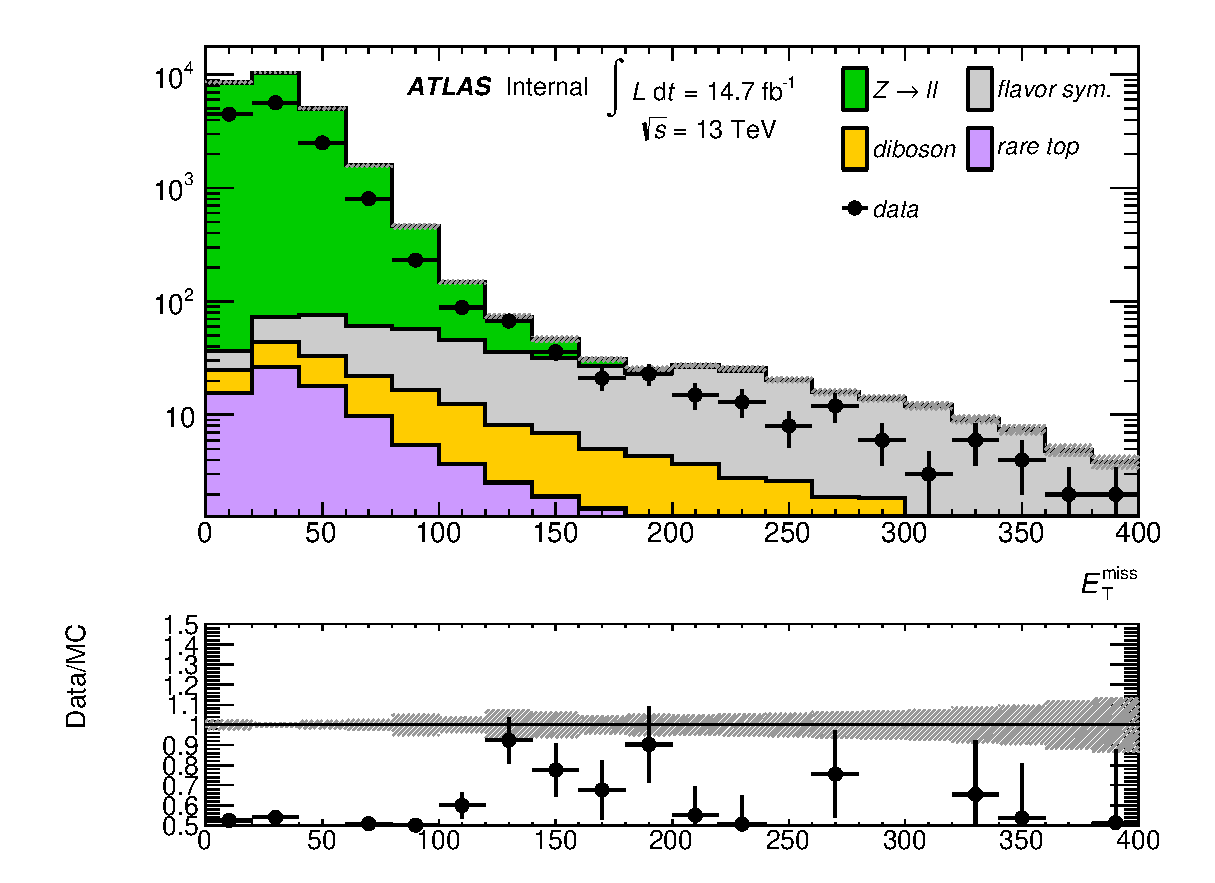
\includegraphics[width=.85\linewidth]{figures/fs/ttbar_met_dependence.eps}
\caption{Comparison of data and \ac{MC} in a selection like SRZ, without the \met cut.}
\label{fig:fs_mc_met}
\end{figure}
\end{centering}

This method is extremely effective as a crosscheck because it uses a completely independent dataset from the flavor symmetry method, and the two methods have very little overlap in dependence on \ac{MC}. They produce consistent results in both SRZ and VRS, as shown in \autoref{tab:fs_comparison}.


\begin{table}[h]
\centering

\begin{tabular}{ccc}
\noalign{\smallskip}\hline\noalign{\smallskip}
Region  & Flavour-symmetry  & Sideband fit  \\
\noalign{\smallskip}\hline\hline\noalign{\smallskip}
SRZ & $33 \pm 4$   &  $29 \pm 7$  \\ [+0.05cm]
VR-S & $99\pm8$        &  $92 \pm 25$  \\ [+0.05cm]
\noalign{\smallskip}\hline\hline
\end{tabular}
\caption{ Comparison of \ac{FS} background predictions from the nominal method, the flavor symmetry method, and the cross-check, the sideband fit method. Uncertainties include statistical and systematic uncertainties in both cases. }
\label{tab:fs_comparison}
\end{table}

%-------------------------------------------------------------------------------------

\section{\dyjets Background}
\label{sec:bg-z}

The \dyjets background is mainly produced by a process called Drell-Yan in which annihilating quark/anti-quark pairs produce a $Z$ boson or a virtual photon. These bosons then decay to two leptons, which, in the case of the $Z$ boson, naturally appear in the $Z$-mass window. The boson typically recoils off a hadronic system, which can satisfy the jet and \HT requirement in SRZ. However, this process rarely produces real \met (though occasionally neutrinos do appear in its hadronic decays), so most events with large amounts of \met are the result of extreme mismeasurement. Because SRZ cuts on the very high \met tails of a $Z$ distribution, a small change in the assumptions about jet resolution or energy scale in \ac{MC} can drastically change the prediction, and a low \dyjets prediction can result in a signal-like peak appearing in the final result. 

Because of this volatility in the \ac{MC} prediction in these high \met tails, a data-driven method is used to estimate this background. The method takes $\gamma$+jets events which, like the \dyjets events, contain one boson recoiling against a hadronic system. These $\gamma$+jets events are then corrected for the kinematic differences between $\gamma$ and $Z$s \cite{ATLAS:2012ema, Chatrchyan:2012qka}. The sample of $\gamma$+jets events is taken from CR-$\gamma$, defined in \autoref{tab:regions-z}. This region is similar to the SRZ selection without the \met requirement, but it vetoes events with leptons and requires at least one photon. Additionally, the $\Delta\phi(\text{jet}_{12},{\boldsymbol p}_{\mathrm{T}}^\mathrm{miss})$ cut in SRZ, which is designed to reduce the background from mismeasured jets, is removed for this region because of its unpredictability at very low values of \met, when the angle of the \met is much less meaningful. 

%TODO what is with the pT miss?

The most significant experimental difference between $Z$ and $\gamma$ events is that $Z$ bosons rapidly decay, in the case of this analysis, to two leptons, which are then be observed by the ATLAS detector. In contrast, the photon is stable, and can be directly detected by ATLAS. This means that the reconstructed $Z$ boson and the directly observed photon have very different energy resolutions.




%-------------------------------------------------------------------------------------

\section{Fake and Non-Prompt Leptons}
\label{sec:bg-fake}

The \textit{fakes} background consists of processes that produce only one lepton, but whose events are otherwise kinematically similar to the \ac{SR}. These processes include semileptonic \ttbar, $W$+jets, and single top processes. Though these processes typically only produce one lepton, they can be reconstructed with two leptons due to a hadron being misidentified as a lepton or due to a real non-prompt lepton resulting from photon conversions or $B$-hadron decays. As such, it includes both events that have been properly reconstructed and many that are included in the \ac{SR} due to imperfect reconstruction. As with the \dyjets background, it is very difficult to predict with \ac{MC} because the flaws in reconstruction are typically less well described by the models used in \ac{MC} production than the successes. Nonetheless, a rough estimate can be made of this background by using \ac{MC}, which indicates that the number of fake events in SRZ is consistent with zero. 

Despite the small predicted contribution in the \ac{SR}, a data-driven method called the \textit{matrix method} is employed to estimate these fake events \cite{SUSY-2013-20}. This method is also used to estimate the fakes contribution to other control and validation regions where their impact is more significant. 

In the matrix method, the quality requirements for signal leptons are loosened to give a selection of baseline leptons (see \autoref{tab:eledef} and \autoref{tab:muondef}), which consist of a higher fraction of fake leptons. In each \ac{CR}, \ac{VR}, or \ac{SR}, the remaining kinematic selections are made on the baseline leptons, and the number of leptons in the region which pass the signal lepton requirements ($N_{pass}$) and the number which fail ($N_{fail}$) are measured. For a 1-lepton selection, these quantities can be used to predict the number of fake events that pass the selection according to:

\begin{equation}
N_{\text{pass}}^{\text{fake}} = \frac{N_{\text{fail}} - (1/\epsilon^{\text{real}} - 1) \times N_{\text{pass}} }{1/\epsilon^{\text{fake}} - 1/\epsilon^{\text{real}}}.
\end{equation}

The efficiencies $\epsilon^\text{real}$ and $\epsilon^\text{fake}$ give the relative identification efficiency from baseline to signal for genuine, prompt leptons and fake and non-prompt leptons, respectively. For a 2-lepton selection, the principle is the same, but the equation is more complicated, requiring a four-by-four matrix to account for possible combinations of real and fake leptons. 


To calculate $\epsilon^\text{real}$, the tag-and-probe method is performed a selection of $Z\rightarrow\ell\ell$ data events, CR-real, described in \autoref{tab:regions-fakes}. In this method, one \textit{tag} lepton passing a signal selection is required, as is another \textit{probe} lepton passing a baseline requirement. Distributions in \mll~for events with a tag and a passing probe and events with a tag and a failing probe are produced and fit, and the efficiency is computed using the ratio acquired from the fit. A comparison of data and \ac{MC} in CR-real can be seen in \autoref{fig:fake_realreg}.
 
\begin{table}[htbp]

\resizebox{1\textwidth}{!}{
 \begin{tabular}{lccccccc} %{\textwidth}{@{\extracolsep{\fill}}lcccccccc}
   \noalign{\smallskip}\hline\noalign{\smallskip}
     {\bf Fakes }   &  {\bf \met}   & {\bf $\HT$}  &  {\bf $n_{\text{jets}}$}  & {\bf $m_{\ell\ell} $} &  {\bf SF/DF}  & {\bf OS/SS} & $n_\ell$\\
     {\bf regions} &  {\bf [\GeV]} & {\bf [\GeV]} &                           & {\bf [\GeV]}          &               &         & \\
   \noalign{\smallskip}\hline\noalign{\smallskip}
   CR-real          &  $-$      &  $\bm{> 200}$  &  $\geq 2$ & {\bf 81--101}    &  $2\ell$ SF  & OS & $2$\\
   CR-fake          &  $\bm{<125}$   &  $-$      &  $-$ & $>12$     &  {\bf $2\ell$ SF/DF}  & {\bf SS} & $\geq2$\\
   \noalign{\smallskip}\hline\noalign{\smallskip}
   \noalign{\smallskip}\hline\noalign{\smallskip}
\end{tabular}
} % end of resizebox
\begin{center}
 \caption{Control regions used to measure efficiencies of real and fake leptons. 
 The flavour combination of the dilepton pair is denoted as either ``SF'' for same-flavour or ``DF'' for different flavour.
The charge combination of the leading lepton pairs are given as ``SS'' for same-sign or ``OS'' for opposite-sign.}
\label{tab:regions-fakes}
\end{center}
\end{table}

\begin{centering}
\begin{figure}[bth]
\myfloatalign
\includegraphics[width=.45\linewidth]{figures/fakes/ee-Cut_Real_TT_HT200-pTsublead_fakes-lin_2016.png}
\includegraphics[width=.45\linewidth]{figures/fakes/mm-Cut_Real_TT_HT200-pTsublead_fakes-lin_2016.png}
\caption{Sub-leading lepton \pT\ for $ee$ (left) and $\mu\mu$ (right) events in the tight-tight region used to measure the real-lepton efficiency for 2016. }
\label{fig:fake_realreg}
\end{figure}
\end{centering}

The fake efficiency, $\epsilon^{fake}$, is determined using the tag-and-probe method in CR-fake, also described in \autoref{tab:regions-fakes}. This region is different from all other regions considered in this analysis because it requires same-sign leptons. Very few processes genuinely produce two same-sign leptons, so this region is enhanced in fake leptons. An upper limit on \met is placed on CR-fake to limit the possible contamination from \ac{BSM} processes. According to \ac{MC}, real, prompt leptons make up about 7\% (11\%) of the baseline electron (muon) sample and about 10\% (61\%) of the signal electron (muon) sample in this region. These real lepton backgrounds are subtracted from the CR-fake yields when calculating the efficiencies. \autoref{fig:fake_fakereg} shows a comparison of data and \ac{MC} in this region.

\begin{centering}
\begin{figure}[htbp]
\centering
\includegraphics[width=.45\textwidth]{figures/fakes/me-Cut_Fake_TT-pTsublead_fakes-lin_2016.png}
\includegraphics[width=.45\textwidth]{figures/fakes/mm-Cut_Fake_TT-pTsublead_fakes-lin_2016.png}
\caption{Sub-leading lepton \pT\ for $\mu e$ (left) and $\mu\mu$ (right) events in the tight-tight region used to measure the fake-lepton efficiency for 2016.}
\label{fig:fake_fakereg}
\end{figure}
\end{centering}

This method is validated in a fakes-rich validation region with a same-sign lepton requirement, \met $\geq$ 50\gev, $\geq$ 2 jets, and a veto on \mll~on the $Z$-mass peak for same flavor channels. The results of this validation can be seen in \autoref{fig:fakes_validation}. With the systematic uncertainties included, the prediction agrees well with the data across a wide range of \mll~values. 

%TODO add this to table

\begin{centering}
\begin{figure}[!htb]
\centering
\includegraphics[width=.45\textwidth]{figures/fakes/ee-CutSSMET_zveto-Mll-lin.pdf}
\includegraphics[width=.45\textwidth]{figures/fakes/mm-CutSSMET_zveto-Mll-lin.pdf}
\includegraphics[width=.45\textwidth]{figures/fakes/em-CutSSMET_zveto-Mll-lin.pdf}
\includegraphics[width=.45\textwidth]{figures/fakes/me-CutSSMET_zveto-Mll-lin.pdf}
\caption{Same sign validation regions in the $ee$ (top left), $\mu\mu$ (top right), $e\mu$ (bottom left) and $\mu e$ (bottom right) channels combining 2015+2016 data. Uncertainty bands include both statistical and systematic uncertainties. \label{fig:fakes_validation}}
\end{figure}
\end{centering}

\section{Diboson and Rare Top Processes}
\label{sec:bg-other}

The remaining backgrounds are diboson processes (excluding $WW$, which is included in the \ac{FS} background) and rare top processes. Dibosons events make up about 30\% of the events in SRZ, while rare top process contributions are much smaller. Both are taken directly from \ac{MC}, with validation regions to confirm the accuracy of the prediction. These regions are described in \autoref{tab:regions-z}, and target different parts of these backgrounds. VR-ZZ is a four-lepton selection designed to select a very pure sample of $ZZ$ events. VR-WZ requires three leptons and makes specific cuts on $m_T$, the transverse mass, and \met in order to select mostly $WZ\rightarrow lll\nu$ events. VR-3L is similar to VR-S, but loosens the \HT and \met cuts and requires at least three leptons. This region is designed to target any $\geq3$-lepton process in a region as kinematically close to SRZ as possible while still maintaining enough events to validate. The makeups of these multilepton validation regions, as well as VRS, are shown in \autoref{tab:VRresults}.



\begin{table}[!htb]
\begin{center}
\setlength{\tabcolsep}{0.0pc}
\resizebox{1\textwidth}{!}{
\begin{tabular*}{\textwidth}{@{\extracolsep{\fill}}lrrrr}
\noalign{\smallskip}\hline\noalign{\smallskip}
                                                                             & VR-S            & VR-WZ        & VR-ZZ          & VR-3L   \\[-0.05cm]
\noalign{\smallskip}\hline\noalign{\smallskip}
Observed events                                                              & $236$            & $698$        & $132$          & $32$ \\
\noalign{\smallskip}\hline\noalign{\smallskip}
%Total expected background events                                             & $223.92 \pm 40.84$   &   $612.97\pm8.65$   &    $139.29\pm4.95$    &    $34.52\pm1.39$ \\
% here the total background uncertainty is updated to the quadrature sum of each bkg uncertainty
Total expected background                                             & $224 \pm 41$   &   $613\pm66$   &    $139\pm25$    &    $35\pm10$ \\
\noalign{\smallskip}\hline\noalign{\smallskip}
  Flavour-symmetric             & $99\pm8$   &   -                &    -                 &    -              \\
  $WZ/ZZ$ events                                                             & $27\pm13$  &   $573\pm66$ &    $139\pm25$        &    $25\pm10$ \\
  Rare top events                                                            & $11\pm3$   &   $14\pm3$   &    $0.44\pm0.11$     &    $9.1\pm2.3$  \\
  \dyjets\ events                                                            & $84\pm37$  &   -                &    -                 &    -              \\
  Fake lepton events                                                         & $4\pm4$    &   $26\pm6$   &    -                 &    $0.6\pm0.3$  \\
 \noalign{\smallskip}\hline\noalign{\smallskip}
\end{tabular*}
} % end of resizebox
\end{center}
\caption{Yields in validation regions. In VRS, data-driven background estimates are used for \dyjets, fakes, and \ac{FS} processes. All other backgrounds are taken from \ac{MC}, including all backgrounds in the multi-lepton \ac{VR}s. Uncertainties include statistical and systematic components. }
\label{tab:VRresults}
\end{table}


To confirm that the kinematics are well modeled in the diboson validation regions, distributions of boson mass and \pt are shown in \ac{MC} and data. Figures \ref{fig:diboson_wz} and \ref{fig:diboson_wz2} show these distributions for VR-WZ, and \autoref{fig:diboson_zz} shows these distributions for VR-ZZ. 

\begin{centering}
\begin{figure}[htbp]
\centering
\includegraphics[width=.9\textwidth]{figures/dibosons/WZ_Wmass.png}
\includegraphics[width=.9\textwidth]{figures/dibosons/WZ_Zmass.png}
\caption{Distribtuions of data and \ac{MC} in VR-WZ. Reconstructed transverse mass of the $W$ (top) and mass of the $Z$ (bottom). \label{fig:diboson_wz}}
\end{figure}
\end{centering}

\begin{centering}
\begin{figure}[htbp]
\centering
\includegraphics[width=.9\textwidth]{figures/dibosons/WZ_Wpt.png}
\includegraphics[width=.9\textwidth]{figures/dibosons/WZ_Zpt.png}
\caption{Distribtuions of data and \ac{MC} in VR-WZ. \pT of the $W$ (top) and $Z$ (bottom). \label{fig:diboson_wz2}}
\end{figure}
\end{centering}

\begin{centering}
\begin{figure}[htbp]
\centering
\includegraphics[width=.9\textwidth]{figures/dibosons/ZZ_Zmass.png}
\includegraphics[width=.9\textwidth]{figures/dibosons/ZZ_Zpt.png}

\caption{Distribtuions in VR-WZ. On the top, mass of the $Z$ bosons in the event, and on the bottom, \pT of the $Z$ bosons. \label{fig:diboson_zz}}
\end{figure}
\end{centering}

 % Background Estimation and Systematic Uncertainty
% Chapter 10

\chapter{Systematic Uncertainties} % Chapter title

\label{ch:backgrounds} 

\section{Uncertainties on Data-Driven Backgrounds}

\subsection{Uncertainties on the Flavor Symmetry Method}
\label{sec:unc_fs}

The flavor symmetry method is a data driven method that makes its estimate primarily on based events populating an \ac{SR}-like \ac{CR} in the different-flavor channel. The statistical uncertainty on these events makes up the dominant uncertainty on the method. To reduce this uncertainty, the \mll~range on the \ac{CR} is expanded, approximately tripling the number of events in CR-FS. The statistical uncertainty is reduced by this expansion, though it is still significantly higher than any of the other systematic uncertainties on this method, as seen in \autoref{tab:fs_errors}. Also included in the statistical uncertainty column is the uncertainty on the number of non-\ac{FS} events in CR-FS, which is used to scale the prediction to account for contamination in the \ac{CR}. 

\begin{table}[!ht]
\begin{center}
 \begin{tabular}{lcc|cccccc}
 \hline 
 \multirow{3}{*}{Reg.}	& \multirow{3}{*}{Ch.} 	& \multirow{3}{*}{Pred.} & \multicolumn{6}{c}{Uncertainties} \\
   \cline{4-9} 
   		 	& 		 	& 	  		& stat.  		& MC 		& k  			& dAOD 		& \mll  	& total \\
   			& 			& 		 	& 			 	& clos. 	& and $\alpha$	& usage	 	& shape  	& \\
   \hline
   \hline
\multirow{3}{*}{SRZ}
& $ee$ & 16.50 & 1.82 & 0.88 & 0.53 & 0.12 & 0.22 & 2.11 \\ 
& $\mu\mu$ & 16.67 & 1.83 & 0.79 & 0.33 & 0.11 & 0.23 & 2.04 \\ 
& $ee$+$\mu\mu$ & 33.16 & 3.66 & 1.07 & 0.86 & 0.23 & 0.45 & 3.94 \\ 
\hline
\multirow{3}{*}{VRS}
& $ee$ & 49.70 & 3.21 & 2.34 & 2.20 & 0.34 & 0.75 & 4.61 \\ 
& $\mu\mu$ & 49.60 & 3.14 & 2.88 & 1.40 & 0.31 & 0.75 & 4.56 \\ 
& $ee$+$\mu\mu$ & 99.31 & 6.34 & 4.00 & 3.60 & 0.65 & 1.49 & 8.47 \\ 
\hline
 
\hline
\hline
 \end{tabular}
\end{center}
 \caption{
   Uncertainties in the on-Z signal and validation regions. Nominal predictions are given with statistical uncertainty (including uncertainty from subtracted backgrounds), MC Closure uncertainty, uncertainty on the prediction from varying $k$ and $\alpha$ by their statistical uncertainties, comparing the efficiencies from AODs to that of DAODs, and on the \mll~widening, which includes MC statistics and a data/MC comparison in a loosened region.
 }
 \label{tab:fs_errors}
\end{table}

The next largest contribution to the uncertainty comes from \ac{MC} closure tests, which are used to determine how effective the method is in its prediction. If, for example, using weights derived from an inclusive selection at high \met lead to a bias, the closure test would indicate that and an appropriate uncertainty could be placed on the estimate based on the difference between the \ac{MC} prediction and the prediction from the flavor symmetry method. 

In this test, the entire \ac{FS} procedure is performed on \ttbar \ac{MC}, including a recalculation of weighting factors $\alpha$ and $k$. The prediction from $e\mu$ events in \ac{MC} is compared to the \ac{MC} $ee$ and $\mu\mu$ events, as seen in \autoref{fig:fs_closure}. The difference between the two predictions is then summed in quadrature with the statistical uncertainty on each prediction to give the total closure uncertainty seen in \autoref{tab:fs_errors}. In these closure tests, all predictions agree within the statistical uncertainty, so the largest contributor to the resulting error is \ac{MC} statistics. 

\begin{centering}
\begin{figure}[!ht]
\myfloatalign
\includegraphics[width=.85\linewidth]{figures/fs/ee+mm_ratio_mll_VRZ_widened.eps}
\includegraphics[width=.85\linewidth]{figures/fs/ee+mm_ratio_mll_SRZ_widened.eps}
\caption{\ac{MC} closure plots of VRS (top) and SRZ (bottom). The number of events from MC (black points) is compared to the number of events predicted from the flavor symmetry method (yellow histogram). The comparison is performed before the expanded \mll~window is used to predict the on-$Z$ bin, but because the shape is taken from the same \ac{MC}, the result is identical.}
\label{fig:fs_closure}
\end{figure}
\end{centering}

A small uncertainty is added based on the statistical uncertainty on the $k$ and $\alpha$ factors derived from data. These factors are measured in many different bins (see, for example, the different measurements of $k$ in \autoref{fig:fs_k}), and as a consequence, some bins can have very large statistical uncertainties. To assess the uncertainty on the total estimate, each measurement of these factors is varied by its uncertainty in order to produce the maximum and minimum possible prediction. The differences with respect to the nominal prediction are used to create a symmetrized error, which is included in \autoref{tab:fs_errors}.

\begin{centering}
\begin{figure}[bth]
\myfloatalign
\includegraphics[width=.85\linewidth]{figures/fs/data_efficiencies_2j_Z_lep0.eps}
\includegraphics[width=.85\linewidth]{figures/fs/data_efficiencies_2j_Z_lep1.eps}
\caption{Measurements of $k$, the ratio of electron to muon events, in bins of $\pT$ and $\eta$. On the top is the measurements indexed by the leading lepton, while the measurements indexed by the subleading lepton are on the bottom. These efficiencies are for the 2016 dataset.}
\label{fig:fs_k}
\end{figure}
\end{centering}

The next uncertainty considers a potential bias in the way the $\alpha$ factors are calculated. Because they are derived from data, there is already trigger dependence in data collection; only events passing a trigger are stored. Additional trigger dependence is created by the data format used for analysis. ATLAS data and \ac{MC} are stored in a format called \ac{AOD}, but smaller, slimmer versions of these datasets, called \acp{dAOD} are used for analysis. These \acp{dAOD} are designed with specific analyses in mind, filtering on the triggers and objects required by the analyses. As a consequence, in the \ac{dAOD} used in this analysis, there are explicit requirements that lepton or \met triggers are passed in order for events to be included. 

As a consequence, the trigger efficiencies $\epsilon^\text{trig}$ used in \autoref{eq:kandalpha} to define $\alpha$ do not consider all possible data events. The $epsilon^\text{trig}$ factor is calculated for each trigger using events passing the kinematic selection for that trigger, outlined in \autoref{sec:trig_strategy}. The efficiency factor is then measured according to the equation

\begin{equation}
\epsilon^\text{trig} = \frac{N_\text{trig}}{N_\text{all}} 
\end{equation}

where $N_\text{trig}$ is the number of events passing the trigger in the kinematic selection and $N_\text{all}$ is all events in the selection. The latter measurement is the one subject to this bias, as it contains only the events that pass at least one trigger required for inclusion in the \ac{dAOD}. As a consequence of these missing events, the $\epsilon^\text{trig}$ values will be artificially high. However, because the ratio of trigger efficiencies for the different channels is the only quantity needed for this analysis, the missing events will only bias the prediction if the different channels are differently impacted by the trigger preselection.

Calculating the flavor symmetry method's dependence on these biases requires the use of \ac{MC}. With a generated \ac{MC} sample, there is no trigger dependence, so an unskimmed sample can be compared to a typical skimmed \ac{MC} \ac{dAOD} to identify the effect of the skimming. \autoref{fig:fs_alpha} shows a comparison of the $\alpha$ factors calculated for different bins in \met from the nominal source, data, as well as these two \ac{MC} sources. A \met dependence would be the most likely bias between the two \ac{MC}-derived $\alpha$ factors because \met triggers are the only triggers besides lepton triggers that will allow an event to be accepted into the dAOD used by this analysis. Though there is some difference between the data-derived $\alpha$ and those taken from \ac{MC}, it is clear from this plot that there is very little dependence on the choice of an unskimmed or skimmed sample. The calculation of the uncertainty is performed by repeating the flavor symmetric method in \ac{MC} with each of the two $\alpha$ factors and using the difference between the estimates as a symmetric error.

\begin{centering}
\begin{figure}[bth]
\myfloatalign
\includegraphics[width=.85\linewidth]{figures/fs/trigger_ratios.eps}
\caption{$\alpha$, the trigger efficiency ratio, calculated as a function of \met from three different sources: data (blue), the usual skimmed \ttbar \ac{MC} (red), and an unskimmed \ttbar \ac{MC} (green).}
\label{fig:fs_alpha}
\end{figure}
\end{centering}

The last uncertainty relates to the main \ac{MC} dependence of the method - the \mll~shape of the \ac{FS} background. A correction factor is taken from \ac{MC} in order to account for the \mll~widening, and the accuracy of that factor must be checked. Its shape is compared to that of data in region similar to VR-FS, but with an \HT cut lowered to 300 \gev~to increase statistics. The difference between the fraction of events on the $Z$-mass peak in data and \ac{MC} in this region is taken as a systematic uncertainty. To confirm that using this lowered \HT cut still gives a valid answer, the fractions are compared as a function of \HT in \autoref{fig:fs_frac_ht}. In these plots, especially in the higher-statistics 2016 plot, it is clear both that the data and \ac{MC} agree very well and that there is no strong \HT dependence. 

\begin{centering}
\begin{figure}[bth]
\myfloatalign
\includegraphics[width=.85\linewidth]{figures/fs/frac_vs_ht_2015.eps}
\includegraphics[width=.85\linewidth]{figures/fs/frac_vs_ht_2016.eps}
\caption{Plots of the fraction of on-Z events with a VR-FS-like selection as a function of \HT. The top figure shows 2015 data and \ac{MC} while the bottom figure shows the same for 2016.}
\label{fig:fs_frac_ht}
\end{figure}
\end{centering}

All the uncertainties are calculated independently for the two datasets, then added together. Statistical uncertainties, including the \ac{MC} closure statistical uncertainties and the $k$ and $\alpha$ uncertainties, are added in quadrature between the two years. Uncertainties that are more likely to be correlated, such as the difference between the two estimates in \ac{MC} closure and the dependence on using a dAOD to calculate trigger efficiencies, are added linearly. The total uncertainty is about 12\% of the nominal prediction in SRZ and about 9\% in VRS. 

%----------------------------------------------------------------------------------------

\subsection{Uncertainties on the $\gamma$+jets Method}

%----------------------------------------------------------------------------------------

\subsection{Uncertainties on the Fakes Background}

Systematic uncertainties on the fakes background are derived from a series of variations on the nominal method.  Variations include scaling the real and fake efficiencies up and down by their statistical uncertainties, scaling the prompt lepton contamination in CR-fake up and down by 20\%, and by requiring and vetoing $b$-tagged jets in CR-fake to determine the dependence on heavy flavor. 
Statistical uncertainties can also be large in regions with small numbers of events in the the baseline selection, such as SRZ. In other regions, the $b$-tagging dependence provides the largest uncertainty. The full breakdown of uncertainties for the most important regions are listed in ~\autoref{tab:syst:fakes_onz1516}.

\begin{table}[htbp]
\centering
\resizebox{\textwidth}{!}{
\begin{tabular}{l|cccccc}
Variation & SRZ & CRT & CRFS & VRFS & VRS & VRT  \\
\hline\hline
Nominal & 0.10 $\pm$ 1.61 & 25.39 $\pm$ 5.35 & 3.73 $\pm$ 2.19 & 10.53 $\pm$ 3.56 & 3.64 $\pm$ 3.20 & 80.06 $\pm$ 9.80   \\
\hline
EL F Up & 0.15  	& 30.23 & 3.96 & 10.93 & 3.56  	& 92.46   \\
EL F Down & 0.06  	& 21.80 & 3.52 & 10.18 & 3.54 	& 70.07   \\
EL R Up & 0.25  	& 26.17 & 3.92 & 11.10 & 4.13 	& 82.57   \\
EL R Down & -0.07  	& 24.51 & 3.52 & 9.92 & 3.10 	& 77.24   \\
MU F Up & -0.20  	& 32.48 & 4.77 & 16.41 & 5.25 	& 86.48   \\
MU F Down & 0.29  	& 20.17 & 2.91 & 7.04 & 2.87 	& 70.12   \\
MU R Up & 0.13 		& 25.67 & 3.78 & 10.66 & 3.81 	& 81.18   \\
MU R Down & 0.05 	& 25.04 & 3.67 & 10.38 & 3.44 	& 78.72   \\
\hline
Total Sys 		& +0.26 -0.35 		& +8.64 -6.39 	& +1.08 -0.87 	& +5.92 -3.56 	& +1.70 -0.97  	& +14.24 -14.42  \\
Total Sys (\%) 	& +261.05 -354.72  	& +34.01 -25.19 & +29.05 -23.23 & +56.22 -33.85 & +46.57 -26.60 & +17.78 -18.02  \\
\hline
Real Cont. Up 	& 0.23 	& 20.97 & 3.06 & 8.08 	& 3.15 	& 68.79   \\
Real Cont. Down & -0.01 & 29.67 & 4.38 & 12.95 	& 4.16 & 90.23   \\
b-jet 			& 0.31 	& 40.44 & 5.28 & 8.98 	& 5.63 & 120.50   \\
no b-jet 		& 0.16 	& 23.44 & 3.08 & 11.38 	& 3.97 & 70.55   \\
\hline
Total Sys & +0.25 -0.11 			& +15.65 -4.83 & +1.69 -0.93 & +2.56 -2.90 & +2.09 -0.49  			& +41.71 -14.74  \\
Total Sys (\%) & +260.46 -109.06 	& +61.66 -19.02 & +45.30 -24.85 & +24.32 -27.58 & +57.31 -13.35 	& +52.10 -18.42  \\
\end{tabular}
}
\caption{ Systematic uncertainties on the fake-lepton background for on-Z regions for 2015+2016 yields. The nominal yield includes statistical uncertainty from the baseline selection in a given region. The following rows indicate the results of varying the real and fake lepton efficiencies up and down by by their statistical uncertainty. Real cont. gives an uncertainty on the the contamination of real leptons in the fake lepton efficiency. $b$-jet and no $b$-jet indicate the impact of requiring or vetoing $b$-tagged jets in the regions used to measure the fake efficiency. \label{tab:syst:fakes_onz1516}}
\end{table}

%----------------------------------------------------------------------------------------

\section{Theoretical and Experimental Uncertainties}

Experimental uncertainties cover any detector effect or \ac{LHC} condition that may not be modeled precisely correctly in \ac{MC}. For each uncertainty, a standard prescription from the ATLAS experiment is followed. Uncertainties are included on the following parameters:  
\begin{itemize}
\item Luminosity (2.9\%) \cite{2011lumi,2012lumi}
\item Jet energy scale \cite{ATL-PHYS-PUB-2015-015}
\item Jet energy resolution \cite{ATL-PHYS-PUB-2015-015}
\item Jet vertex tagging
\item Heavy flavor tagging
\item \met soft term \cite{ATL-PHYS-PUB-2015-023}
\item $e/\mu$ momentum scale  
\item $e/\mu$ trigger, reconstruction, and identification efficiencies
\item Pile-up
\end{itemize}

These uncertainties are applied to all \ac{MC} samples used in the analysis. This includes signal models, diboson and rare top samples for the nominal estimate, and all backgrounds taken from \ac{MC} in the sideband fit. 

Theoretical uncertainties include cross-section uncertainties, scale uncertainties, and \ac{PDF} uncertainties. For the diboson samples, the scale uncertainties, given in \autoref{table:Diboson_theoryuncert} are calculated by varying each scale up and down by a factor of two. These are combined with a 6\% cross-section uncertainty and a generator uncertainty obtained by comparing {\sc Powheg} and {\sc Sherpa} \ac{MC} yields in a given region. This generator uncertainty, shown in \autoref{table:Diboson_powhegsherpa1}, is dominant in most regions. Rare top processes are given a $13\%$ PDF and scale variation uncertainty \cite{Alwall:2014hca} and a $22\%$ cross section uncertainty \cite{Campbell:2012,Lazopoulos:2008,Garzelli:2012bn}. 

\begin{table}
	\begin{center}
 		\begin{tabular}{l|c|c|c|c|c|c|c}
		    \hline \hline 
   			\multicolumn{3}{c}{$VV \rightarrow ll\nu\nu$ Samples} \\
  	 		\hline
			&	SRZ & VRS & CRT & VRT & VRWZ & VRZZ & VR3L \\
			\hline
			resummation & 0.07 & 0.03 & 0.01 & 0.02 & 0.00 & 0.00 & 0.00 \\
			renormalization & 0.13 & 0.17 & 0.16 & 0.22 & 0.00 & 0.00 & 0.00 \\
			factorization & 0.01 & 0.01 & 0.01 & 0.03 & 0.00 & 0.00 & 0.00 \\
			total & 0.15 & 0.17 & 0.16 & 0.22 & 0.00 & 0.00 & 0.00 \\
		    \hline 
   			\multicolumn{3}{c}{$WZ \rightarrow lll\nu$ Samples} \\
  	 		\hline
			&	SRZ & VRS & CRT & VRT & VRWZ & VRZZ & VR3L \\
			\hline
			resummation & 0.07 & 0.05 & 0.13 & 0.08 & 0.02 & 0.00 & 0.01 \\
			renormalization & 0.26 & 0.20 & 0.28 & 0.21 & 0.07 & 0.00 & 0.18 \\
			factorization & 0.04 & 0.04 & 0.02 & 0.06 & 0.01 & 0.00 & 0.02 \\
			total & 0.28 & 0.21 & 0.31 & 0.23 & 0.07 & 0.00 & 0.18 \\
  	 		\hline
   			\multicolumn{3}{c}{$ZZ \rightarrow llll$ Samples} \\
  	 		\hline
			&	SRZ & VRS & CRT & VRT & VRWZ & VRZZ & VR3L \\
			\hline
			resummation & 0.27 & 1.07 & 0.01 & 0.01 & 0.06 & 0.01 & 0.53 \\
			renormalization & 0.28 & 0.26 & 0.30 & 0.60 & 0.07 & 0.04 & 0.14 \\
			factorization & 0.27 & 0.25 & 0.30 & 0.58 & 0.13 & 0.02 & 0.16 \\
			total & 0.48 & 1.13 & 0.43 & 0.84 & 0.16 & 0.05 & 0.57 \\
  	 		\hline
 		\end{tabular}
	\end{center}
	\caption{Fractional uncertainties of dibosons in signal and validation regions from Sherpa scale variations.}
	\label{table:Diboson_theoryuncert}
\end{table}

\begin{table}
\begin{center}
\begin{tabular}{c|c|c|c|c|c} \\
Region & Sherpa & Sherpa & Powheg & Powheg & \% \\
& Events/fb$^{-1}$ & Events & Events/fb$^{-1}$ & Events & Difference \\
\hline
\hline
\multicolumn{6}{c}{WZ Samples} \\
\hline
SRZ+VRZ & 5.219 & 76.722 & 3.286 & 48.300 & 37.046 \\
CRT+VRT & 1.060 & 15.583 & 0.742 & 10.913 & 29.970 \\
\hline
\multicolumn{6}{c}{WW/ZZ Samples} \\
\hline
SRZ+VRZ & 1.921 & 28.244 & 0.685 & 10.070 & 71.424 \\
CRT+VRT & 6.281 & 92.332 & 3.142 & 46.188 & 55.474 \\
\hline
\end{tabular}
\end{center}
\caption{Comparison of yields in on-$Z$ and off-$Z$ regions in Sherpa and Powheg diboson MC at $14.7~\mathrm{fb}^{-1}$.}
\label{table:Diboson_powhegsherpa1}
\end{table}

Signal models have both the central value and uncertainty on cross-sections taken from an envelope of predictions using different scales and \ac{PDF} sets \cite{Kramer:2012bx}. The signal processes are calculated at \ac{NLO+NLL}; they are initially callculated at \ac{NLO} in the strong coupling constant, with additional terms from next-to-leading-logarithmic resummation of soft gluon emission \cite{Beenakker:1996ch,Kulesza:2008jb,Kulesza:2009kq,Beenakker:2009ha,Beenakker:2011fu}.


%----------------------------------------------------------------------------------------

\section{Impact of Uncertainties on the Signal Region}


The breakdown of each major uncertainty's contribution to the total uncertainty in SRZ is shown in \autoref{tab:syst}. The dominant uncertainty is the diboson generator uncertainty, followed by the statistical uncertainty from the \ac{FS} background. Uncertainties smaller than 1\% are not shown in the table. 

\begin{table}[h]
\centering
\small
\begin{tabular}{lc}
\noalign{\smallskip}\hline\noalign{\smallskip}
Source  & Relative systematic uncertainty [\%] \\
\noalign{\smallskip}\hline\noalign{\smallskip}
 & SRZ \\
\noalign{\smallskip}\hline\noalign{\smallskip}
Total systematic uncertainty & 17    \\ 
\noalign{\smallskip}\hline
$WZ/ZZ$ generator uncertainty  & 13  \\
Flavour symmetry (statistical) & 7              \\
$WZ/ZZ$ scale uncertainty      & 6   \\
\dyjets\ (systematic)          & 4   \\
Flavour symmetry (systematic)  & 3      \\
\dyjets\ (statistical)         & 2   \\
Fake-leptons                   & 1   \\
\noalign{\smallskip}\hline
\end{tabular}
\caption{
Overview of the dominant sources of systematic uncertainty on the total background estimate in the signal regions.
The values shown are relative to the total background estimate, shown in \%.}
\label{tab:syst}
\end{table}

%---------------------------------------------------------------------------------------- % Background Estimation and Systematic Uncertainty
% Chapter 11

\chapter{Results} % Chapter title

\label{ch:results} 

The results of the search can be seen in \autoref{tab:results}, which displays the expected and observed numbers of events in SRZ, both divided by channel and inclusively. The predictions and uncertainties for each background are shown, though many of these uncertainties are correlated between backgrounds, so the final uncertainty does not correspond to a simple addition in quadrature of each error. A total of sixty events are observed, with 53.5 $\pm$ 9.3 events expected. \autoref{fig:results_plot} shows the expected and observed results visually for the \ac{SR} as well as three \acp{VR}, all designed to verify the accuracy of the backgrounds taken from \ac{MC}. Excellent agreement is seen in all cases, with the largest deviation at about $1\sigma$. 

\begin{centering}
\begin{figure}[!hbt]
\myfloatalign
\includegraphics[width=.9\linewidth]{figures/results/makeSummaryPlot_linear.pdf}
\caption{Comparison of background predictions and data yields in four validation regions, as well as the signal region. Definitions of all regions can be found in \autoref{tab:regions-z}, with both rare top and fake backgrounds grouped together under the ``other'' label. The uncertainty band includes all statistical and systematic uncertainties. Below is a panel of the one-sided statistical significances of the deviations between the predicted and observed quantities for each region.}
\label{fig:results_plot}
\end{figure}
\end{centering}

\begin{sidewaystable*}
\caption{
Number of events expected and observed in the $ee$, $\mu\mu$, and combined channels. Expected predictions include all systematic and statistical uncertainties discussed in \autoref{ch:background_uncertainties}. Also shown is the discovery $p$-value for zero signal strength ($p(s=0)$)~\cite{Baak:2014wma}, Gaussian significance, 95\% \ac{CL} observed and expected upper limits on the number of signal events ($S^{95}$), and the corresponding observed upper limit on the visible cross section ($\langle\epsilon\sigma\rangle^{95}_\text{obs}$).
}
\begin{center}
\setlength{\tabcolsep}{0.0pc}
%%
\begin{tabular*}{\textwidth}{@{\extracolsep{\fill}}lccc}
\noalign{\smallskip}\hline\noalign{\smallskip}
                                                                            & SRZ                 & SRZ $ee$      & SRZ $\mu\mu$  \\[-0.05cm]
\noalign{\smallskip}\hline\noalign{\smallskip}
%%
Observed events                                                             & $60$                     & $35$                   &   $25$ \\
\noalign{\smallskip}\hline\noalign{\smallskip}
%%
Total expected background events                                            & $53.5 \pm 9.3$         & $27.1 \pm 5.1$       &   $26.8 \pm 4.4$ \\
\noalign{\smallskip}\hline\noalign{\smallskip}
%%
  Flavour-symmetric (\ttbar, $Wt$, $WW$ and $Z\rightarrow\tau\tau$) events  & $33.2 \pm 3.9$         & $16.5 \pm 2.1$       &   $16.7 \pm 2.0$       \\
%%
  \dyjets\ events                                                           & $\makebox[3ex]{\hfill 3.1} \pm \makebox[2ex]{2.8\hfill}$          & $1.0_{-1.0}^{+1.3}$ &   $\makebox[3ex]{\hfill 2.1} \pm \makebox[2ex]{1.4\hfill}$     \\
%%
  $WZ/ZZ$ events                                                            & $14.2 \pm 7.7$         & $\makebox[3ex]{\hfill 7.8} \pm \makebox[2ex]{4.3\hfill}$        &   $\makebox[3ex]{\hfill 6.4} \pm \makebox[2ex]{3.5\hfill}$        \\
%%
  Rare top events                                                           & $\makebox[3ex]{\hfill 2.9} \pm \makebox[2ex]{0.8\hfill}$          & $\makebox[3ex]{\hfill 1.4} \pm \makebox[2ex]{0.4\hfill}$        &   $\makebox[3ex]{\hfill 1.5} \pm \makebox[2ex]{0.4\hfill}$  \\
%%
 Fake-lepton events                                                         & $\makebox[3ex]{\hfill 0.1}_{-0.1}^{+0.8}$   & $0.5_{-0.5}^{+0.7}$ &   $\makebox[3ex]{\hfill 0}^{+0.2}$    \\
 \noalign{\smallskip}\hline\noalign{\smallskip}
$p(s=0)$                                                                    & 0.32      & 0.15        & 0.5        \\
Significance $(\sigma)$                                                               & 0.47                     & 1.00                   & 0           \\
Observed (Expected) $S^{95}$                                                & 28.2 ($24.5_{-6.7}^{+8.9}$) & 22.0 ($15.8_{-4.5}^{+6.5}$) & 12.9 ($14.0_{-3.9}^{+5.7}$) \\
$\langle\epsilon\sigma\rangle^{95}_\text{obs}$~[fb]                         & 1.9             & 1.5                    & 0.88   \\
 \noalign{\smallskip}\hline\noalign{\smallskip}
\end{tabular*}
\end{center}
\label{tab:results}
\end{sidewaystable*}

\autoref{tab:results} also shows several statistical interpretations of the results. The discovery $p$-value for zero signal strength, which gives the probability that the observed events are compatible with a \ac{SM}-only hypothesis, is given as 0.32. The significance is listed as 0.47 $\sigma$, which is a reinterpretation of the $p$-value into a gaussian significance. This $p$-value is one-sided; when the data yield is less than expected the $p$-value is set to 0.5, and the significance is set to 0. $S^{95}$, the upper limit on the number of signal events that could be in the \ac{SR} at a 95\% \ac{CL}, is determined both for the expected and observed number of events. This limit is also reinterpreted based on the integrated luminosity used in the seach to produce an upper limit on the visible cross-section of signal events, $\langle\epsilon\sigma\rangle^{95}_\text{obs}$.

The predictions in SRZ, combined with \mll~shapes taken from \ac{MC}, are used to produce plots in a broader \mll~range, seen in \autoref{fig:results_widemll}. These plots are useful demonstrations of efficacy of the background estimation methods, showing the well-modeled \dyjets shape in the same-flavor region, and in the different-flavor region, demonstrating that there are no extreme fluctuations within the region used to predict the flavor symmetric background.

\begin{centering}
\begin{figure}[!hbt]
\myfloatalign
\includegraphics[width=.48\linewidth]{figures/results/mll_SF_R_a_SCALED.eps}
\includegraphics[width=.48\linewidth]{figures/results/mll_DF_R_a_SCALED.pdf}
\caption{Comparisons as a function of \mll~of background predictions with observed data in an SRZ-like region, with the \mll~cut removed. Left is the same-flavor channel, where all background shapes are taken from \ac{MC} and scaled to their SRZ predictions, except for the \dyjets background, which is taken entirely from the data-driven background. Right is the different-flavor channel, in which the backgrounds are taken directly from \ac{MC}, except for \ttbar, which is scaled to match the total data yield. }
\label{fig:results_widemll}
\end{figure}
\end{centering}

Focusing in on the \ac{SR} itself, comparisons of background predictions, observed events, and signal models can be made as a function of key variables for the analysis. \autoref{fig:results_srdists} shows several of these. The first two figures focus on the features of the \ac{SR} events' leading leptons; they give the mass and \pt of a hypothetical parent particle reconstructed from the leptons. In the case of events with a real $Z$ boson, these variables simply give that boson's mass at \pt. The next two figures show distributions in the two most important variables used to differentiate signal from background, \met and \HT. In this analysis, where the frozen \ac{SR} resulted in cuts on these quantities that are lower than those that would be chosen based on a new optimization, these plots show that, even in more sensitive regions, no large excess above the \ac{SM} background is seen. The last pair of figures relates to the jets in the event, showing the total number of jets and the total number of $b$-jets in the \ac{SR} events. The $b$-jet quantity is not explicitly cut on in the analysis because the fraction of $b$-jets produced is extremely model dependent. However, an excess at high $b$-jet multiplicity would suggest a \ac{BSM} process. In each of these distributions, the observed distributions match the background predictions very well, and no evidence for any of the superimposed signal models is seen. 

\begin{centering}
\begin{figure}[!hbt]
\myfloatalign
\includegraphics[width=.48\linewidth]{figures/results/mll_ee_mm_srz_R_a.eps}
\includegraphics[width=.48\linewidth]{figures/results/Zpt_ee_mm_srz_R_a.eps}
\includegraphics[width=.48\linewidth]{figures/results/met_ee_mm_srz_R_a.eps}
\includegraphics[width=.48\linewidth]{figures/results/htincl_ee_mm_srz_R_a.eps}
\includegraphics[width=.48\linewidth]{figures/results/njets_ee_mm_srz_R_a.eps}
\includegraphics[width=.48\linewidth]{figures/results/nbjets_ee_mm_srz_R_a.eps}
\caption{ Distributions of observed data, background predictions, and simulated signals are shown in SRZ as a function of \mll, $\pt^{\ell\ell}$, \met, \HT, number of jets, and number of $b$-jets. The two example signals have $(m(\tilde{g}),m(\tilde{\chi}^{0}_{2}))=(1095, 205)$~\GeV. All background shapes are taken from \ac{MC}, and in the case of flavor symmetric and \dyjets backgrounds, their yields are scaled to match the data-driven predictions. Uncertainties include statistical and systematic components.}
\label{fig:results_srdists}
\end{figure}
\end{centering}

Comparisons of the observed and expected yield are also made as a function of $\Delta\phi(\text{jet}_{12},{\boldsymbol p}_{\mathrm{T}}^\mathrm{miss})$, shown in \autoref{fig:results_dphi}. Here, results are shown in a region similar to SRZ with the cut on this variable removed, showing the efficacy of the background prediction in a region enhanced in \dyjets events. Again, excellent agreement is seen between the background prediction and observed data.

\begin{centering}
\begin{figure}[!hbt]
\myfloatalign
\includegraphics[width=.9\linewidth]{figures/results/dPhi_azmet_ee+mm_onz_SR.eps}
\includegraphics[width=.9\linewidth]{figures/results/dPhi_azmet_ee+mm_onz_VR.eps}
\caption{Comparisons as a function of $\Delta\phi(\text{jet}_{12},{\boldsymbol p}_{\mathrm{T}}^\mathrm{miss})$ of background predictions with observed data in an SRZ-like (left) and VRS-like (right) region, with the $\Delta\phi(\text{jet}_{12},{\boldsymbol p}_{\mathrm{T}}^\mathrm{miss})$ cut removed. All background shapes are taken from \ac{MC} and scaled to their SRZ predictions, except for the \dyjets background, which is taken entirely from the data-driven background.}
\label{fig:results_dphi}
\end{figure}
\end{centering}

%----------------------------------------------------------------------------------------
 % Results
% Chapter 12

\chapter{Interpretations} % Chapter title
\label{ch:interpretations} 

Using the simplified models discussed in \autoref{sec:simplified_models}, these results can be interpreted into exclusions of theories based on the masses of the particles involved. Of course, these exclusions include all the assumptions of the models used, so they shouldn't be interpreted to mean that no theory with a given set of particle masses can possibly exist, but they do provide a helpful guideline for targeting future searches and comparing results from different analyses.

Limits are determined using a program called HistFitter \cite{Baak:2014wma}, designed within the ATLAS experiment, which builds upon the capabilities of ROOT \cite{BRUN199781}, RooStats \cite{1009.1003}, and HistFactory \cite{Cranmer:2012sba} to combine the uncertainties of the various background predictions, including their correlations, and produce cross-section limits at 95\% \ac{CL} using the $CL_{\text{S}}$ prescription~\cite{statforumlimits,clsread}. In this prescription, a likelihood is constructed based on the expected signal and background contributions to the \ac{SR}. Nuisance parameters are created based on the statistical and systematic uncertainties for each data-driven background, as well as for each systematic applied to the \ac{MC}-driven background estimates. The fit uses Gaussian models for nuisance parameters for all signal and background uncertainties, except for the flavor symmetry method and the \ac{MC}-based backgrounds, which are interpreted as Poissonian. Experimental uncertainties are considered fully correlated across the signal and background \ac{MC}-based estimates. 

A fit is performed, leaving a signal strength parameter ($\mu$) free, to maximize the likelihood, and subsequent fits are preformed to at discrete $\mu$ values to determine the relative likelihood of each value. Using this relative likelihood, the probability of a background-only hypothesis, $p_b$, can be determined by setting $\mu=0$, as well as the probability of a signal + background hypothesis $p_{s+b}$ with any non-zero signal strength, but nominally with $\mu=1$. The confidence limit is constructed as a ratio

\begin{equation}
CL_S = \frac{p_{s+b}}{1-p_b}. 
\end{equation}

Then, if $CL_S$ falls below 5\%, the signal + background hypothesis can be excluded at 95\%. Expected exclusion limits are constructed by assuming the observed data precisely matches the prediction, and 1$\sigma$ uncertainty bands are formed by varying ????????. The observed limit uses the actual observation of data in the \ac{SR} to set exclusion limits, so any excess above the expected background will result in worse limits than expected, and any deficit will result in better limits. This exclusion is displayed with error bands that represent the theoretical uncertainty on the signal models. 

\begin{figure}[!htb]
\centering
\includegraphics[width=.8\textwidth]{figures/interpretation/excl_SM_GG_N2_1.eps}
\includegraphics[width=.8\textwidth]{figures/interpretation/excl_SM_SS_N2.eps}  
\caption{
Expected and observed exclusion contours derived from the results in SRZ for the (top) $\tilde{g}$--$\chitwozero$ on-shell grid and (bottom) $\tilde{q}$--$\chitwozero$ on-shell grid. 
The dashed blue line indicates the expected limits at $95\%$ CL and the yellow band shows the $1\sigma$ variation of the expected limit as a consequence of the uncertainties in the background prediction and the experimental uncertainties in the signal ($\pm1\sigma_\text{exp}$). 
The observed limits are shown by the solid red line, with the dotted red lines indicating the variation resulting from changing the signal cross section within its uncertainty ($\pm1\sigma^\text{SUSY}_\text{theory}$). \label{fig:excl_SMGGN2_1}
}
\end{figure}


\begin{figure}[htbp]
\centering
\includegraphics[width=.8\textwidth]{figures/interpretation/excl_SM_GG_N2.eps}
\caption{
Expected and observed exclusion contours derived from the results in SRZ for the $\tilde{g}$--$\chionezero$ on-shell grid. 
The dashed blue line indicates the expected limits at $95\%$ CL and the yellow band shows the $1\sigma$ variation of the expected limit as a consequence of the uncertainties in the background prediction and the experimental uncertainties in the signal ($\pm1\sigma_\text{exp}$). 
The observed limits are shown by the solid red line, with the dotted red lines indicating the variation resulting from changing the signal cross section within its uncertainty ($\pm1\sigma^\text{SUSY}_\text{theory}$).
\label{fig:excl_SMGGN2}
}
\end{figure}

%----------------------------------------------------------------------------------------
 % Interpretation

\cleardoublepage % Empty page before the start of the next part

%------------------------------------------------

\ctparttext{This section presents conclusions and an outlook for future work.} % Text on the Part 2 page describing the content in Part 2

\part{Conclusions} % Second part of the thesis

% Chapter 13

\chapter{Conclusions} % Chapter title

\label{ch:conc} 

%----------------------------------------------------------------------------------------
 % Conclusions
% Chapter 14

\chapter{Outlook} % Chapter title

\label{ch:outlook} 

%----------------------------------------------------------------------------------------
 % Outlook

\cleardoublepage % Empty page before the start of the next part

%----------------------------------------------------------------------------------------
%	THESIS CONTENT - APPENDICES
%----------------------------------------------------------------------------------------

\appendix

\part{Appendix} % New part of the thesis for the appendix

\include{Chapters/Chapter0A} % Appendix A
%\include{Chapters/Chapter0B} % Appendix B - empty template

%----------------------------------------------------------------------------------------
%	POST-CONTENT THESIS PAGES
%----------------------------------------------------------------------------------------

\cleardoublepage\include{FrontBackMatter/Bibliography} % Bibliography

%\cleardoublepage\include{FrontBackMatter/Declaration} % Declaration

%\cleardoublepage\include{FrontBackMatter/Colophon} % Colophon

%----------------------------------------------------------------------------------------

\end{document}
